%%%%%%%%%%%%%%%%%%%%%%%%%%%%%%%%%%%%%%%%%
% Beamer Presentation
% LaTeX Template
% Version 1.0 (10/11/12)
%
% This template has been downloaded from:
% http://www.LaTeXTemplates.com
%
% License:
% CC BY-NC-SA 3.0 (http://creativecommons.org/licenses/by-nc-sa/3.0/)
%
%%%%%%%%%%%%%%%%%%%%%%%%%%%%%%%%%%%%%%%%%

%----------------------------------------------------------------------------------------
%	PACKAGES AND THEMES
%----------------------------------------------------------------------------------------
\documentclass{beamer}

\mode<presentation> {

% The Beamer class comes with a number of default slide themes
% which change the colors and layouts of slides. Below this is a list
% of all the themes, uncomment each in turn to see what they look like.

% \usetheme{default}
%\usetheme{AnnArbor}
%\usetheme{Antibes}
%\usetheme{Bergen}
%\usetheme{Berkeley}
%\usetheme{Berlin}
%\usetheme{Boadilla}
% \usetheme{CambridgeUS}
%\usetheme{Copenhagen}
\usetheme{Darmstadt}
%\usetheme{Dresden}
%\usetheme{Frankfurt}
%\usetheme{Goettingen}
%\usetheme{Hannover}
%\usetheme{Ilmenau}
%\usetheme{JuanLesPins}
%\usetheme{Luebeck}
%\usetheme{Madrid}
%\usetheme{Malmoe}
%\usetheme{Marburg}
%\usetheme{Montpellier}
%\usetheme{PaloAlto}
%\usetheme{Pittsburgh}
%\usetheme{Rochester}
%\usetheme{Singapore}
%\usetheme{Szeged}
%\usetheme{Warsaw}

% As well as themes, the Beamer class has a number of color themes
% for any slide theme. Uncomment each of these in turn to see how it
% changes the colors of your current slide theme.

%\usecolortheme{albatross}
%\usecolortheme{beaver}
%\usecolortheme{beetle}
%\usecolortheme{crane}
%\usecolortheme{dolphin}
%\usecolortheme{dove}
%\usecolortheme{fly}
%\usecolortheme{lily}
%\usecolortheme{orchid}
%\usecolortheme{rose}
%\usecolortheme{seagull}
%\usecolortheme{seahorse}
%\usecolortheme{whale}
%\usecolortheme{wolverine}

%\setbeamertemplate{footline} % To remove the footer line in all slides uncomment this line
%\setbeamertemplate{footline}[page number] % To replace the footer line in all slides with a simple slide count uncomment this line

%\setbeamertemplate{navigation symbols}{} % To remove the navigation symbols from the bottom of all slides uncomment this line
}

% tikz and flowchart
\usepackage{tikz}
\usetikzlibrary{shapes.geometric, arrows}

\usepackage{transparent}
\usepackage{overpic}
\usepackage{subfig}
\usepackage{graphicx} % Allows including images
\usepackage{booktabs} % Allows the use of \toprule, \midrule and \bottomrule in tables
\definecolor{olivegreen}{RGB}{34,139,34}
\definecolor{darkorange}{RGB}{255,140,0}
%----------------------------------------------------------------------------------------
%	TITLE PAGE
%----------------------------------------------------------------------------------------

\title[$\gamma$-ray Earth's Limb analysis]{Study of cosmic-ray spectrum using $\gamma$-ray data from \textit{Fermi} Large Area Telescope (\textit{Fermi}-LAT)} % The short title appears at the bottom of every slide, the full title is only on the title page
% \logo{
\includegraphics[height=0.75cm]{santa}}
\author{Patomporn Payoungkhamdee } % Your name
\institute[MU] % Your institution as it will appear on the bottom of every slide, may be shorthand to save space
{
Mahidol University \\ % Your institution for the title page
\medskip
\textit{patomporn.pay@gmail.com} % Your email address
}
\date{15 July 2018} % Date, can be changed to a custom date

\newcommand{\nologo}{\setbeamertemplate{logo}{}}

\begin{document}

{\nologo
\begin{frame}
\titlepage % Print the title page as the first slide
\end{frame}
}

\begin{frame}
\frametitle{Overview} % Table of contents slide, comment this block out to remove it
\tableofcontents % Throughout your presentation, if you choose to use \section{} and \subsection{} commands, these will automatically be printed on this slide as an overview of your presentation
\end{frame}

%----------------------------------------------------------------------------------------
%	PRESENTATION SLIDES
%----------------------------------------------------------------------------------------


%------------------------------------------------
%    1 ) Background
%------------------------------------------------
\section{Introduction}
% \section{Background}
\subsection{Background}
%---- 1.1 ) What is CRs ---
\begin{frame}
\frametitle{What are cosmic rays}
  \begin{columns}
      \column{0.5\textwidth}

      \begin{figure}
      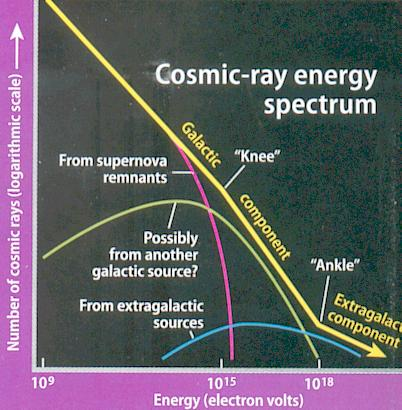
\includegraphics[height=0.7\textheight, width=0.9\textwidth]{CRFeature}
      \caption{Cosmic ray feature : retrieved from  universe-review.ca }
      \end{figure}

      \column{0.5\textwidth}
      \begin{itemize}
      \item{A high-energey particles that travelling through space}
      \\ 
      \item{\textbf{Criteria :} When we call flux it means differential flux}
      \\ 
      \item{\textbf{Feature :} CRs spectrum in rigidity follow power law }
      \item{Discontinuity in spectrum came from superposition of different acceleration mechanism}
      \end{itemize}
  \end{columns}
\end{frame}
%---- Intro objective (PAMELA & AMS) ---
\begin{frame}
\frametitle{Trend in cosmic ray research}
In 2015, the AMS collaboration claims that there is a broken in cosmic ray proton spectrum around 336 GV.
\begin{figure}
  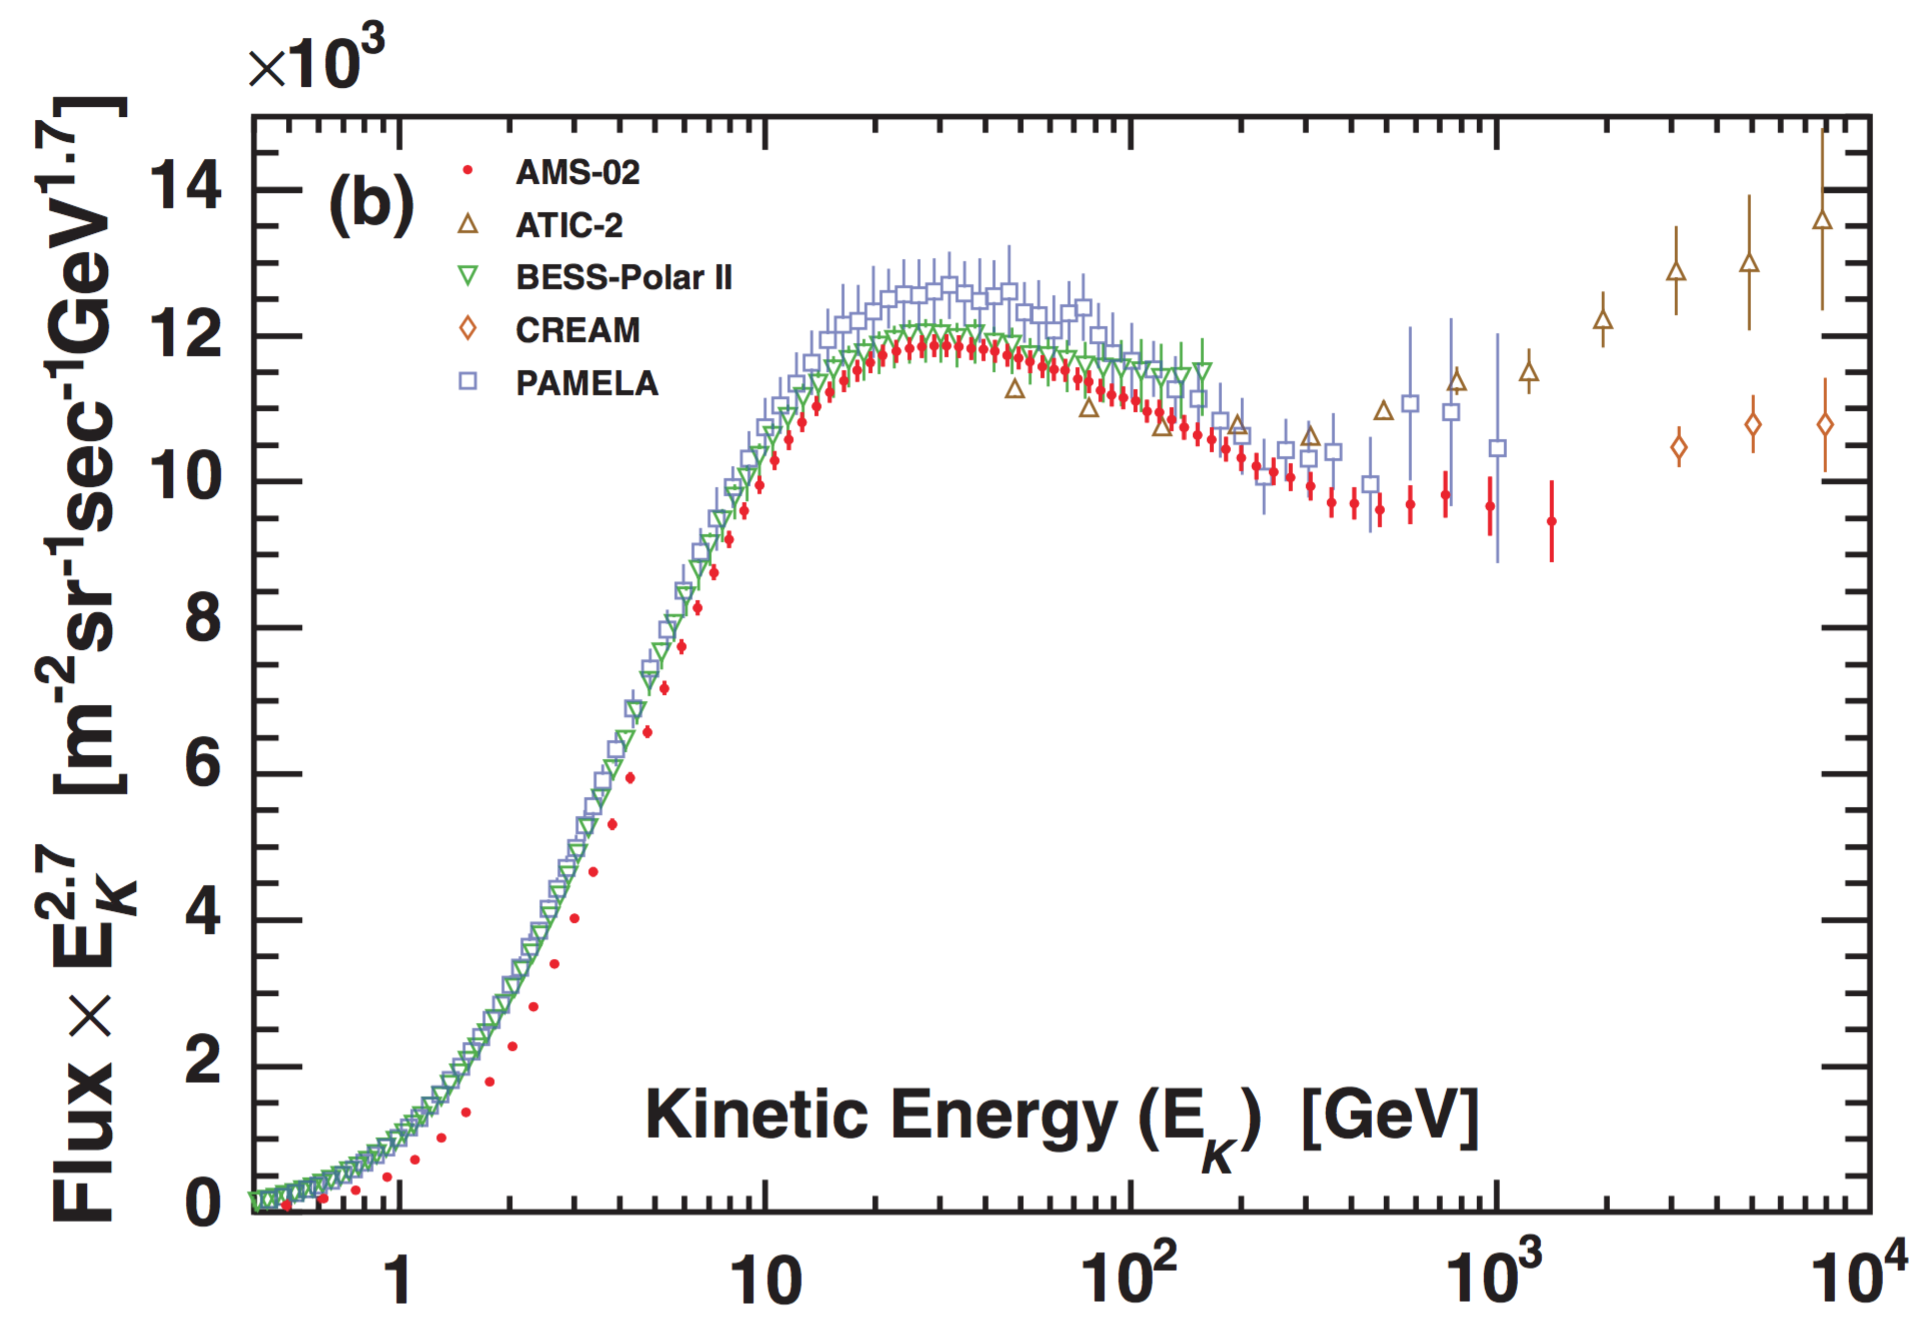
\includegraphics[width=0.6\textwidth]{proton_spectrum}
  \caption{Cosmic rays proton flux : retrieved from M. Aguilar et al. (2015)}
\end{figure}
\end{frame}

%------------------------------------------------
%      2 ) Objectives
%------------------------------------------------
\subsection{Objectives}
% \section{Objectives} % Sections can be created in order to organize your presentation into discrete blocks, all sections and subsections are automatically printed in the table of contents as an overview of the talk

%---- our point ---
\begin{frame}
\frametitle{Objective}
\begin{itemize}
  \item Want to \textcolor{blue}{measure cosmic ray proton spectrum in range GV} by using
  $\gamma$-ray data from \textit{Fermi}-LAT through Kachelrie$\beta$ and Ostapchenko model
  \item Some intruments claim that cosmic ray proton spectrum has discontinuity around 200-350 GV
  , then if our result agree with other intruments. Space \textcolor{blue}{might have another acceleration mechanism that people did not know very well.}
\end{itemize}
\end{frame}

%------     Production schematics --------------
\subsection{Schematics of limb $\gamma$-ray production}
\begin{frame}
\frametitle{Schematics of limb $\gamma$-ray production}
\centering
\begin{figure}[h!]
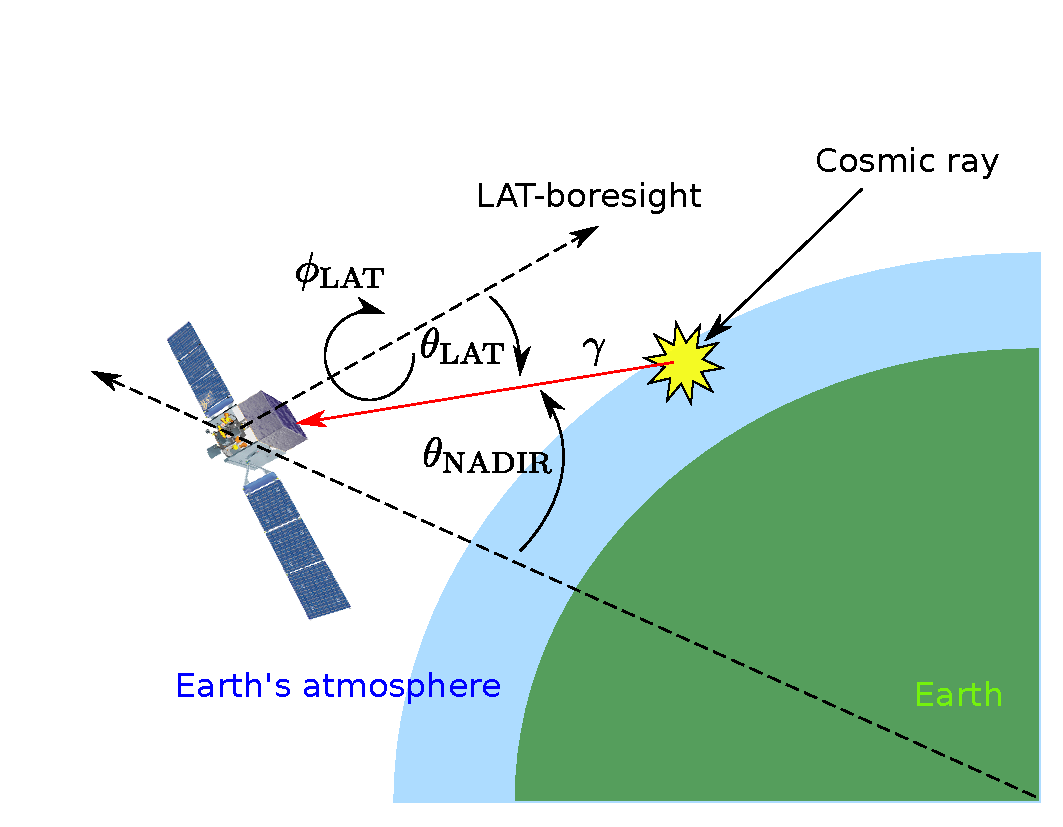
\includegraphics[width = 0.8\textwidth]{lat_production_schematic}
\end{figure}
\end{frame}


%------------------------------------------------
%    3 ) Flux extraction
%------------------------------------------------
\section{Flux extraction}
%------------------------------------------------
%    3.2 ) Data set
%------------------------------------------------
\subsection{Data set}

\begin{frame}
\frametitle{Data selection}
\begin{itemize}
  \item P8R2\_ULTRACLEANVETO\_V6 data from 07/08/2008 to 28/01/2015 ($\sim$7 years) %Use P8R2\_ULTRACLEANVETO\_V6 data which collect only photon
  \item Collect photon energy range from 10 GeV up to 1 TeV
  \item $\theta_{\text{NADIR}}$ $\in$ 68.4$^\circ$  - 70$^\circ$ (Earth's limb)
  \item Use $\theta_{\text{LAT}} < 70^\circ$
\end{itemize}
\end{frame}
%------------------------------------------------
%    3.3 ) Flux calculation
%------------------------------------------------
\subsection{Calculation}
%--- How to calculate flux ---
\begin{frame}
\frametitle{Calculation method}
\begin{enumerate}
  \item Make 2D histogram as much as energy bin that we want
  \item Select photon data and fill in the 2D histogram
  \item Calculate exposure maps which incldue effective area
  and time that LAT view can looking at Earth's limb
  \\ \textbf{Flux} = $\frac{dF}{dE} = \frac{\int_{\text{Limb region}(\text{Count map}/\text{Exposure map})}}{\Delta\Omega\Delta E }$
  \item Divide every single grid of couple histogram (count map and exposure map)
  \item Sum over limb region of this map then divided by solidangle and energy bin width
  \item Now we got $\gamma$-ray flux
\end{enumerate}
\end{frame}
% %--- cntmap ---
% \begin{frame}
% \frametitle{Count map}

% %\begin{figure}[h!]
% %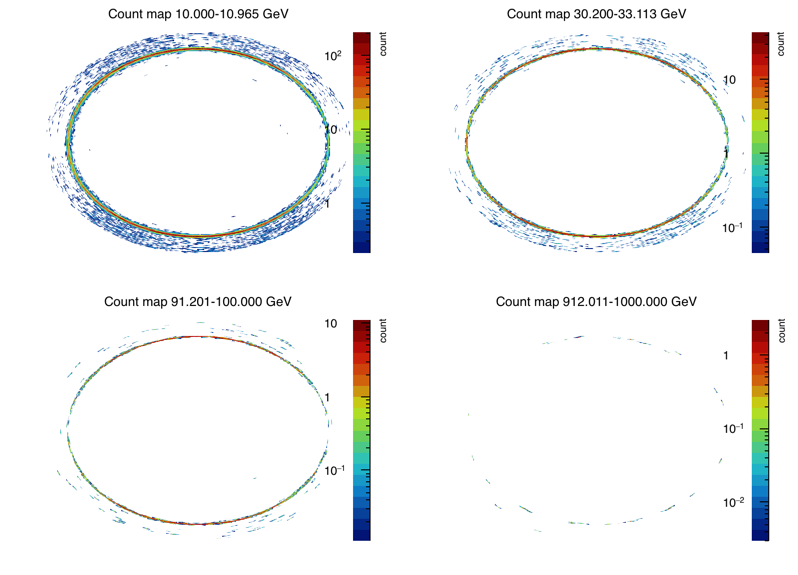
\includegraphics[width = 0.9\textwidth]{cntmap}
% %\caption{Bla1}
% %\end{figure}

% \begin{figure}[h!]
% \begin{tikzpicture}
% \node (0,0) {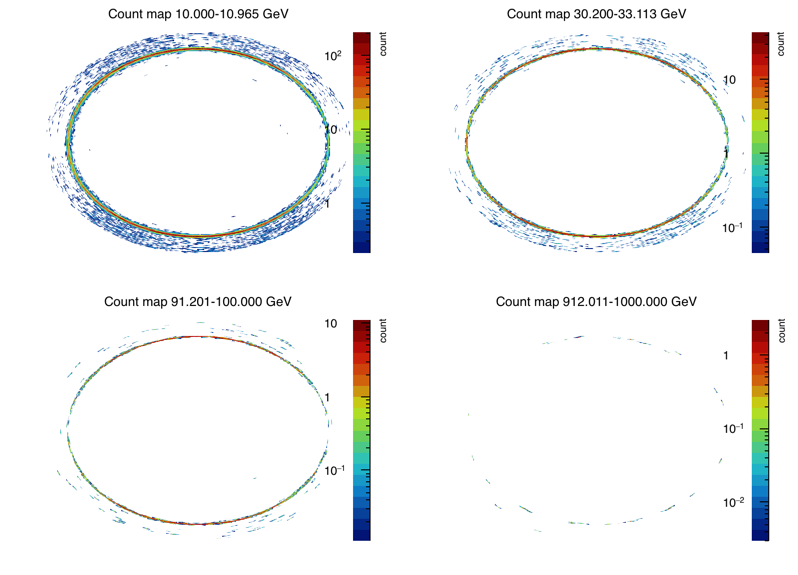
\includegraphics[width=0.9\textwidth]{cntmap}};
% \node [opacity=0.2] (0,0) {\rotatebox{45}{\scalebox{3.5}{\textcolor{red}{preliminary}}}};
% \end{tikzpicture}
% \end{figure}

% \end{frame}
% %--- expmap ---
% \begin{frame}
% \frametitle{Exposure map}

% %\begin{figure}[h!]
% %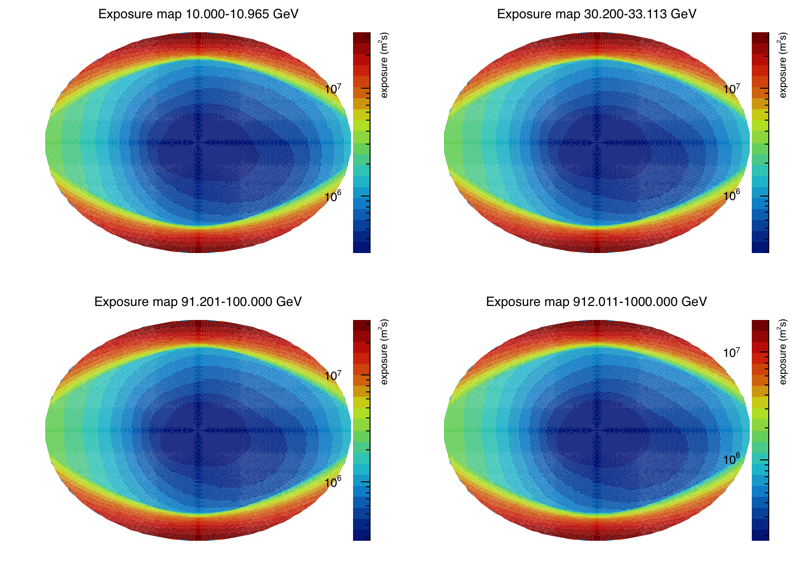
\includegraphics[width = 0.9\textwidth]{expmap}
% %\caption{Bla1}
% %\end{figure}

% \begin{figure}[h!]
% \begin{tikzpicture}
% \node (0,0) {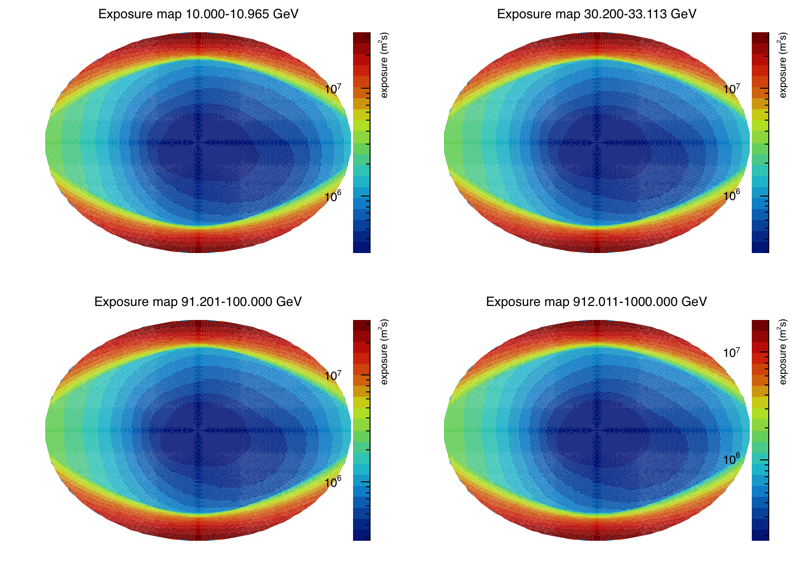
\includegraphics[width=0.9\textwidth]{expmap}};
% \node [opacity=0.2] (0,0) {\rotatebox{45}{\scalebox{3.5}{\textcolor{red}{preliminary}}}};
% \end{tikzpicture}
% \end{figure}

% \end{frame}

% %--- flxmap ---
% \begin{frame}
% \frametitle{Flux map}

% %\begin{figure}[h!]
% %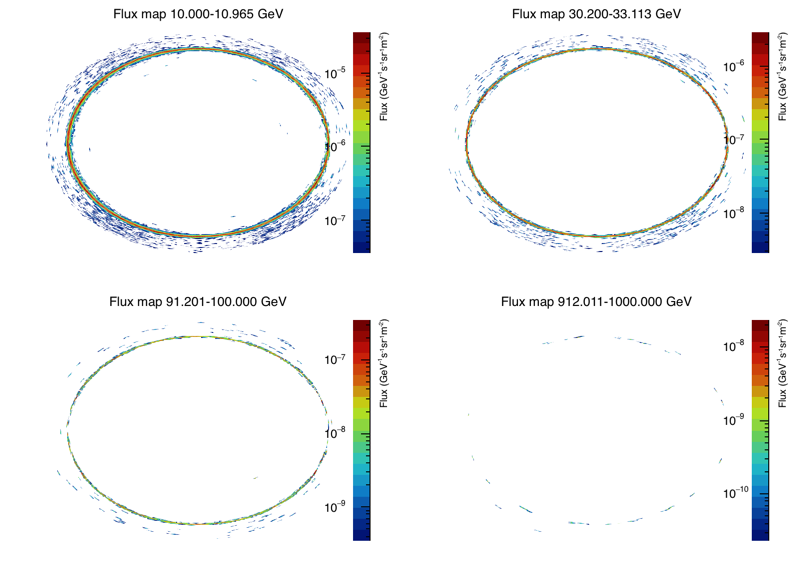
\includegraphics[width = 0.9\textwidth]{flxmap}
% %\caption{Bla1}
% %\end{figure}

% \begin{figure}[h!]
% \begin{tikzpicture}
% \node (0,0) {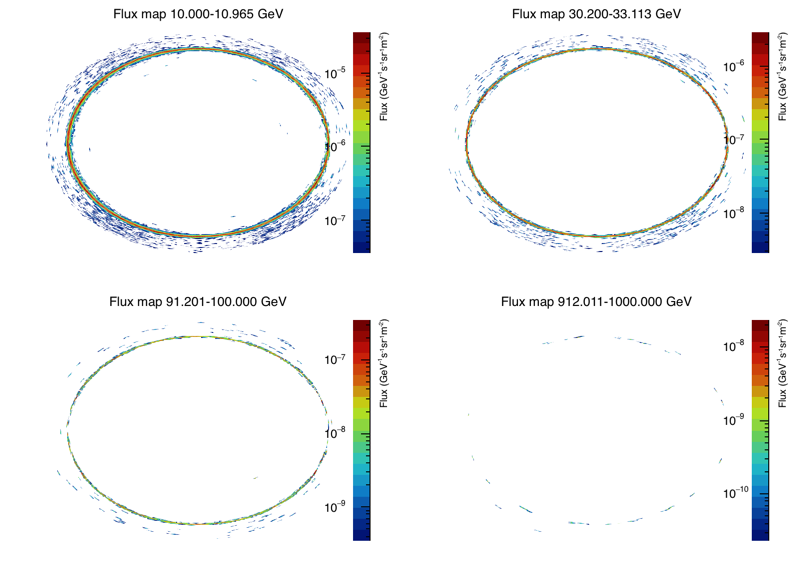
\includegraphics[width=0.9\textwidth]{flxmap}};
% \node [opacity=0.2] (0,0) {\rotatebox{45}{\scalebox{3.5}{\textcolor{red}{preliminary}}}};
% \end{tikzpicture}
% \end{figure}

% \end{frame}

%--- got spectrum ---
\begin{frame}
\frametitle{$\gamma$-ray spectrum from measurement}

%\begin{figure}[h!]
%\includegraphics[width = 0.7\textwidth]{FluxfromExposure}
%\end{figure}

\begin{figure}[h!]
\begin{tikzpicture}
\node (0,0) {\includegraphics[width=0.7\textwidth]{FluxfromExposure}};
\node [opacity=0.2] (0,0) {\rotatebox{45}{\scalebox{2.5}{\textcolor{red}{preliminary}}}};
\node [opacity=1.0] at (2.4,-2.40) {\tiny E (GeV)};
\end{tikzpicture}
\end{figure}
Notice that error bar came from statistics error and the red band already take into account
instrument error
\end{frame}

%------------------------------------------------
%    4 ) Analysis
%------------------------------------------------
\section{Analysis}

% ------- poewr law in rigidity -------------
\subsection{Power law spectrum}
\begin{frame}
  \frametitle{Power law (in rigidity)}
  Typically, cosmic ray spectrum follow power law in rigidity as \\
  \textbf{Single power law (SPL)}
  \begin{equation}
  \frac{dN}{dR} = R_0R^{-\gamma}
  \end{equation}
  \textbf{Broken power law (BPL)}
  \begin{equation}
  \frac{dN}{dR}=
    \begin{cases}
      R_0R^{-\gamma_1}\ :\ E < E_{\text{Break}}\\
      R_0[R(E_{\text{Break}})]^{\gamma_2-\gamma_1}R^{-\gamma_2}\ :\ E \ge E_{\text{Break}}
    \end{cases}
  \end{equation}
  Note for someone who not familiar with rigidity : it just defined by $R\equiv P/q$ when $P, q$ is a momentum and charge of particle
  \end{frame}
%------------------------------------------------
%    4.1 ) K&O model
%------------------------------------------------
\subsection[K$\&$O model]{Kachelrie$\beta$ and Ostapchenko model}
\begin{frame}
\frametitle{Kachelrie$\beta$ and Ostapchenko model}
Is the model which can compute spectrum of $\gamma$-ray from a known incident proton
\begin{equation}
  \small
  \frac{dN_{\gamma}}{dE} \propto \sum_{E_{\text{inc,i}}}\left[\frac{E_{\text{inc,i}}}{E_{\gamma\text{,i}}}\Delta(E_{\text{inc,i}}) \right]\left[ f_{pp}\textcolor{red}{\frac{dN_\text{H}}{dE_{\text{inc,i}}}}\left\{ 1+\textcolor{olivegreen}{\frac{\sigma_{\text{HeN}}}{\sigma{pN}}}\left(\textcolor{red}{\frac{dN_{\text{H}}}{dR}}\right)^{-1} \textcolor{blue}{\frac{dN_{\text{He}}}{dR}} \frac{dR_{\text{He}}}{dR_{\text{H}}}  \right\}\right]
\end{equation}
\begin{itemize}
  \item Red color terms is using for \textcolor{red}{incident proton spectrum}
  \item \textcolor{blue}{Use helium spectrum from AMS-02 measurement (2015)}
  \item $f_{pp}\equiv E_\gamma(d\sigma^{pp\rightarrow\gamma}/dE_\gamma)$ is a table in K$\&$O model which behave like a scattering amplitude
  that depend on the energy of incident particle
  \item Crossection \textcolor{olivegreen}{$\sigma_{\text{HeN}}/\sigma_{pN}$} at high energy ($>$ 10GeV) is almost remain constant ($\approx 1.6$)
\end{itemize}

\end{frame}
%------------------------------------------------
%    4.1 Optimization
%------------------------------------------------
\subsection{Optimization}
\begin{frame}
\frametitle{Poisson likelihood function}
On the previous slide, we want to find the incident proton. \\
Let define some loss function to compare model and measurement
\begin{equation}
  \mathcal{L} = \prod_{i=1}^{N} P_{\text{pois}}(n_{\text{i,model}}, n_{\text{i,measurement}})
\end{equation}

For numerically convenient, redefined into logarithmic form
\begin{equation}
  \log\mathcal{L} \equiv \sum_{i=1}^{N} -\log P_{\text{pois}}(n_{\text{i,model}}, n_{\text{i,measurement}})
\end{equation}
This part is the hard work of computer to find best incident cosmic ray proton that match the
spectrum from measurement.

\end{frame}

%-- Flow chart ---%
  % Define block styles
  \tikzstyle{decision} = [diamond, draw, fill=red!10, 
  text width=2em, text badly centered, node distance=2.5cm, inner sep=0pt]
  \tikzstyle{block} = [rectangle, draw, fill=blue!10, 
  text width=5em, text centered, rounded corners, minimum height=2em]
  \tikzstyle{longblock} = [rectangle, draw, fill=blue!10, 
  text width=10em, text centered, rounded corners, minimum height=4em]
  \tikzstyle{line} = [draw,thick, -latex']
  \tikzstyle{cloud} = [draw, ellipse,fill=red!20, node distance=3cm,
  minimum height=4em]

\begin{frame}\frametitle{Algorithm}

\begin{figure}[!h]
\centering
\begin{tikzpicture}[node distance = 6em, auto]
    \node [block, fill=black!10] (powerlaw) {powerlaw spectrum of proton in rigidity};
    \node [block, right of = powerlaw, node distance = 12em] (model) {$\gamma$-ray spectrum from model};
    \node [block, right of = model] (measurement) {$\gamma$-ray spectrum from measurement};
    \node [block, below left of = measurement, node distance = 8em] (pois) {Poisson likelihood function};
    \node [block, below of = powerlaw] (varyPar) {Apply gradient to parameters $\gamma$, $R_0$};
    \node [decision, below of = varyPar, fill = blue!10] (bestfit) {Best fit?};
    \node [block, right of = bestfit, node distance = 10em, fill = red!10] (return) {Return best fit parameters};

    \path [line] (powerlaw) -- node [anchor=south] {K\&O model} (model);
    \path [line] (model) -- (pois);
    \path [line] (measurement) -- (pois);
    \path [line] (pois) -- (bestfit);
    \path [line] (bestfit) -- node [anchor=east] {No} (varyPar);
    \path [line] (varyPar) -- (powerlaw);
    \path [line] (bestfit) -- node [anchor=north] {Yes} (return);
\end{tikzpicture}
\caption{Flow chart of optimization process}
\end{figure}

\end{frame}

%------------------------------------------------
%    4.3 ) Results
%------------------------------------------------
\section{Results}
\begin{frame}
\frametitle{Results}
\begin{table}
\begin{tabular}{l | c | c | c}
  Best fits & $\gamma_1$ & $\gamma_2$ & $E_{\text{Break}}$ (GeV) \\
  \hline \hline
  SPL & 2.68 $\pm$ 0.01(0.03) & - & -  \\
  BPL & 2.84 $\pm$ 0.04(0.06) & 2.64 $\pm$ 0.04(0.17) & 328 $\pm$ 151(267)
%  & $\gamma_1$ & $\gamma_2$ & $E_{\text{Break}}$ (GeV) \\
% \hline \hline
% Single power law (SPL) & 2.68 & - & -  \\
% Broken power law (BPL) & 2.84 & 2.64 & 328
\end{tabular}
\caption{Optimization results}
\end{table}
\begin{itemize}
  \item Likelihood Ratio Test (LRT) $\Rightarrow$ BPL better than SPL with a significant level of \textcolor{olivegreen}{$3.3\sigma$}
\end{itemize}
\small Where 1$\sigma$ of systematic error and total error (take into account instrumental error) was shown in the table consequently. \newline
% Event though the log-likelihood value of BPL less than SPL but not significantly enough to say cosmic ray proton would be BPL.
Notice that error of parameters came from \textcolor{blue}{Monte Carlo Simulation}
\end{frame}

% --- graph gamma ray
\begin{frame}
\frametitle{$\gamma$-ray spectrum}

\begin{figure}
  \begin{tikzpicture}
  \node (0,0) {\includegraphics[width=0.8\textwidth]{ModelvsMeasurement}};
  \node [opacity=0.2] (0,0) {\rotatebox{45}{\scalebox{2.5}{\textcolor{red}{preliminary}}}};
  \node [opacity=1.0] at (2.7,-2.75) {\tiny E (GeV)};
  \end{tikzpicture}
\end{figure}


\end{frame}
% --- spectrum proton
\begin{frame}
  \frametitle{Proton spectrum}
  
  \begin{figure}[h!]
  \begin{tikzpicture}
  \node (0,0) {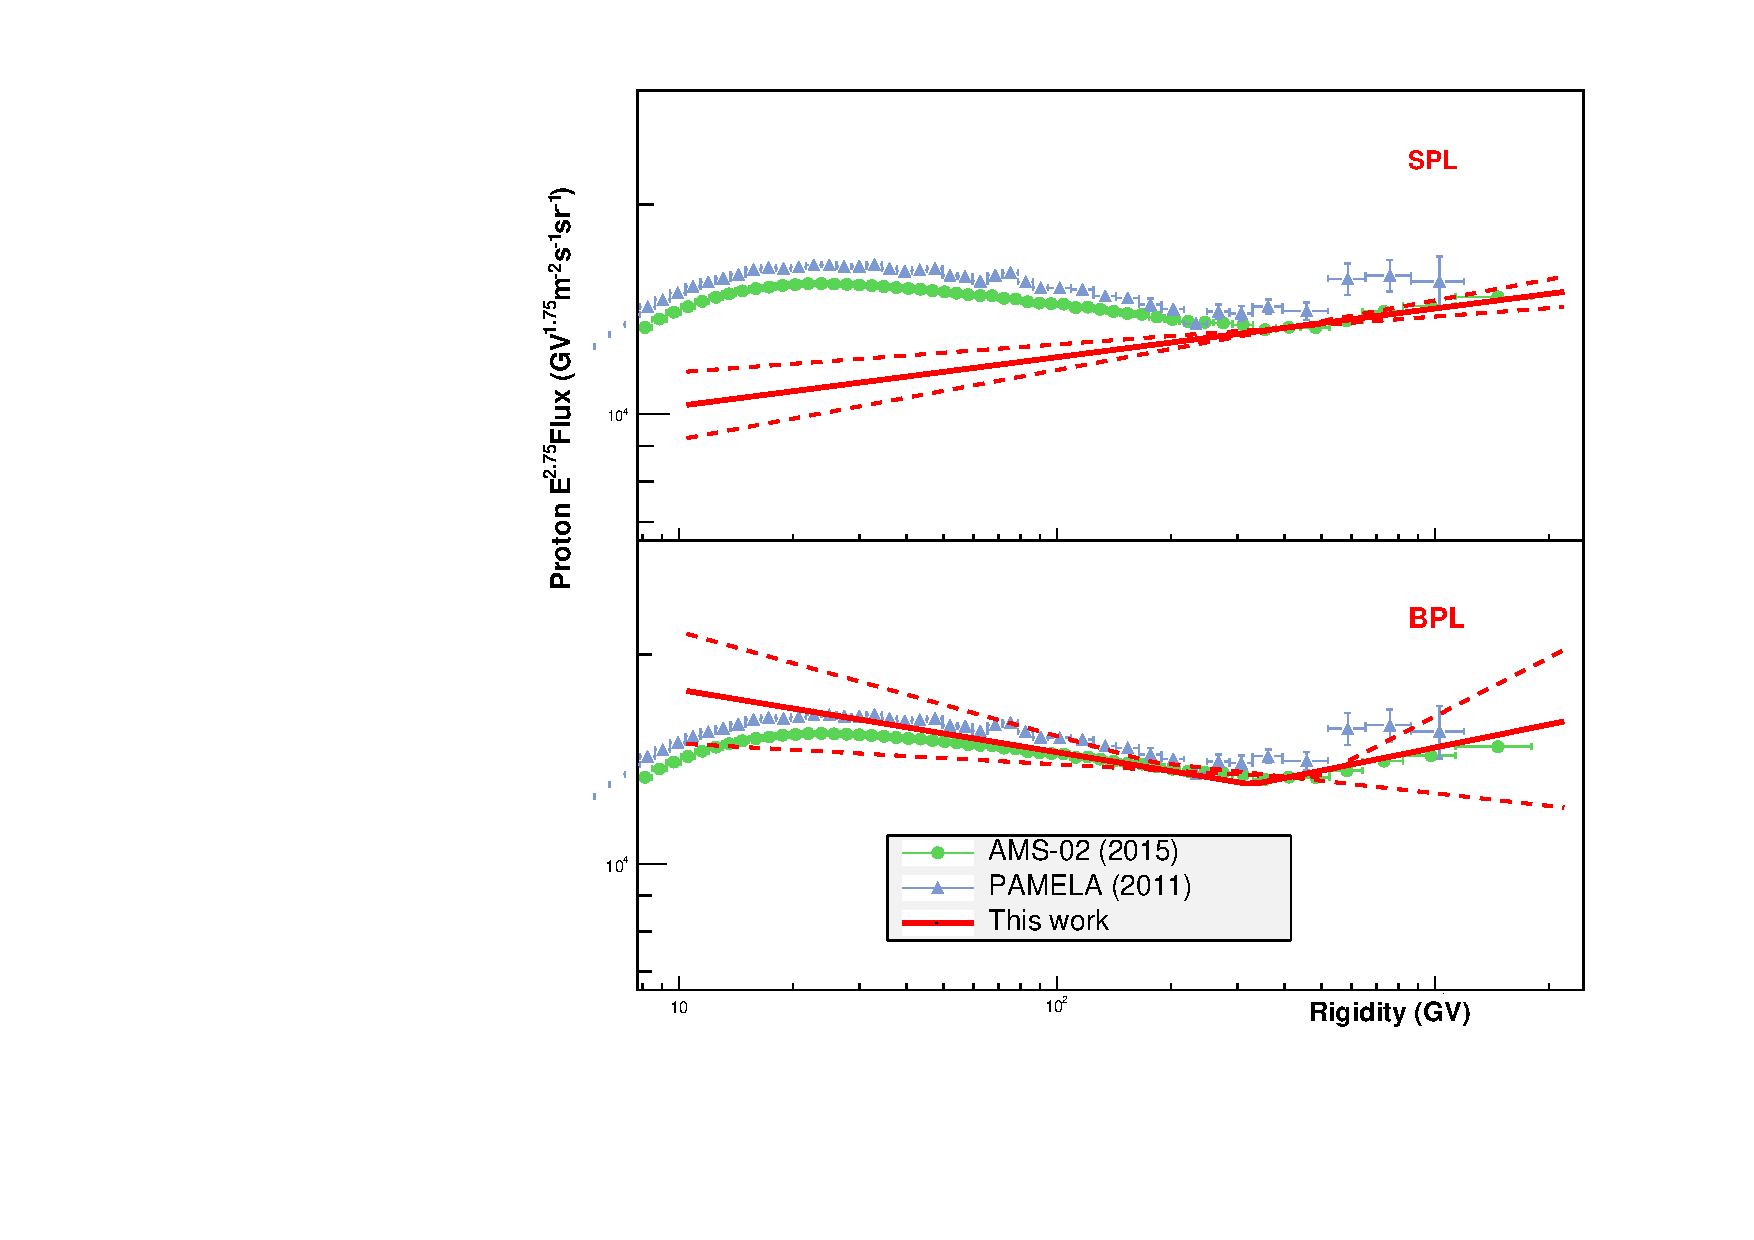
\includegraphics[width=0.8\textwidth]{ProtonSpectrumModelMeasurement}};
  \node [opacity=0.2] (0,0) {\rotatebox{45}{\scalebox{2.5}{\textcolor{red}{preliminary}}}};
  \end{tikzpicture}
  \end{figure}
  
  \end{frame}
%------------------------------------------------
%    4.4 ) Monte carlo Simulation
%------------------------------------------------
% \subsection{Monte Carlo simlation}
% %----- How to deal with this ?
% \begin{frame}
% \frametitle{Error determination}
% \textbf{Statictical error (Random error)}
% \begin{enumerate}
%   \item Get back to raw count and
%   \textcolor{blue}{random new count in each energy bin by Poisson random function}
%   \item Recalculate proton spectrum
%   \item Optimize it and store the parameter that we got
%   \item do it over thoundsand time and fill in histogram to interpret error by saying sigma of gaussian function
% \end{enumerate}
% \textbf{Total error (take into account instrument)}
% \begin{enumerate}
%   \item Get back to raw count and
%   \textcolor{blue}{random new count in each energy bin by Poisson random function}
%   \item \textcolor{blue}{Random value we got again by systematic error (Apparatus)}
%   \item Recalculate proton spectrum
%   \item Optimize it and store the parameter that we got
%   \item do it over thoundsand time and fill in histogram to interpret error by saying sigma of gaussian function
% \end{enumerate}
% \end{frame}

% %----- SPL ------
% \begin{frame}
% \frametitle{Single power law (SPL)}

% \begin{figure}[h!]
% \begin{tikzpicture}
% \node (0,0) {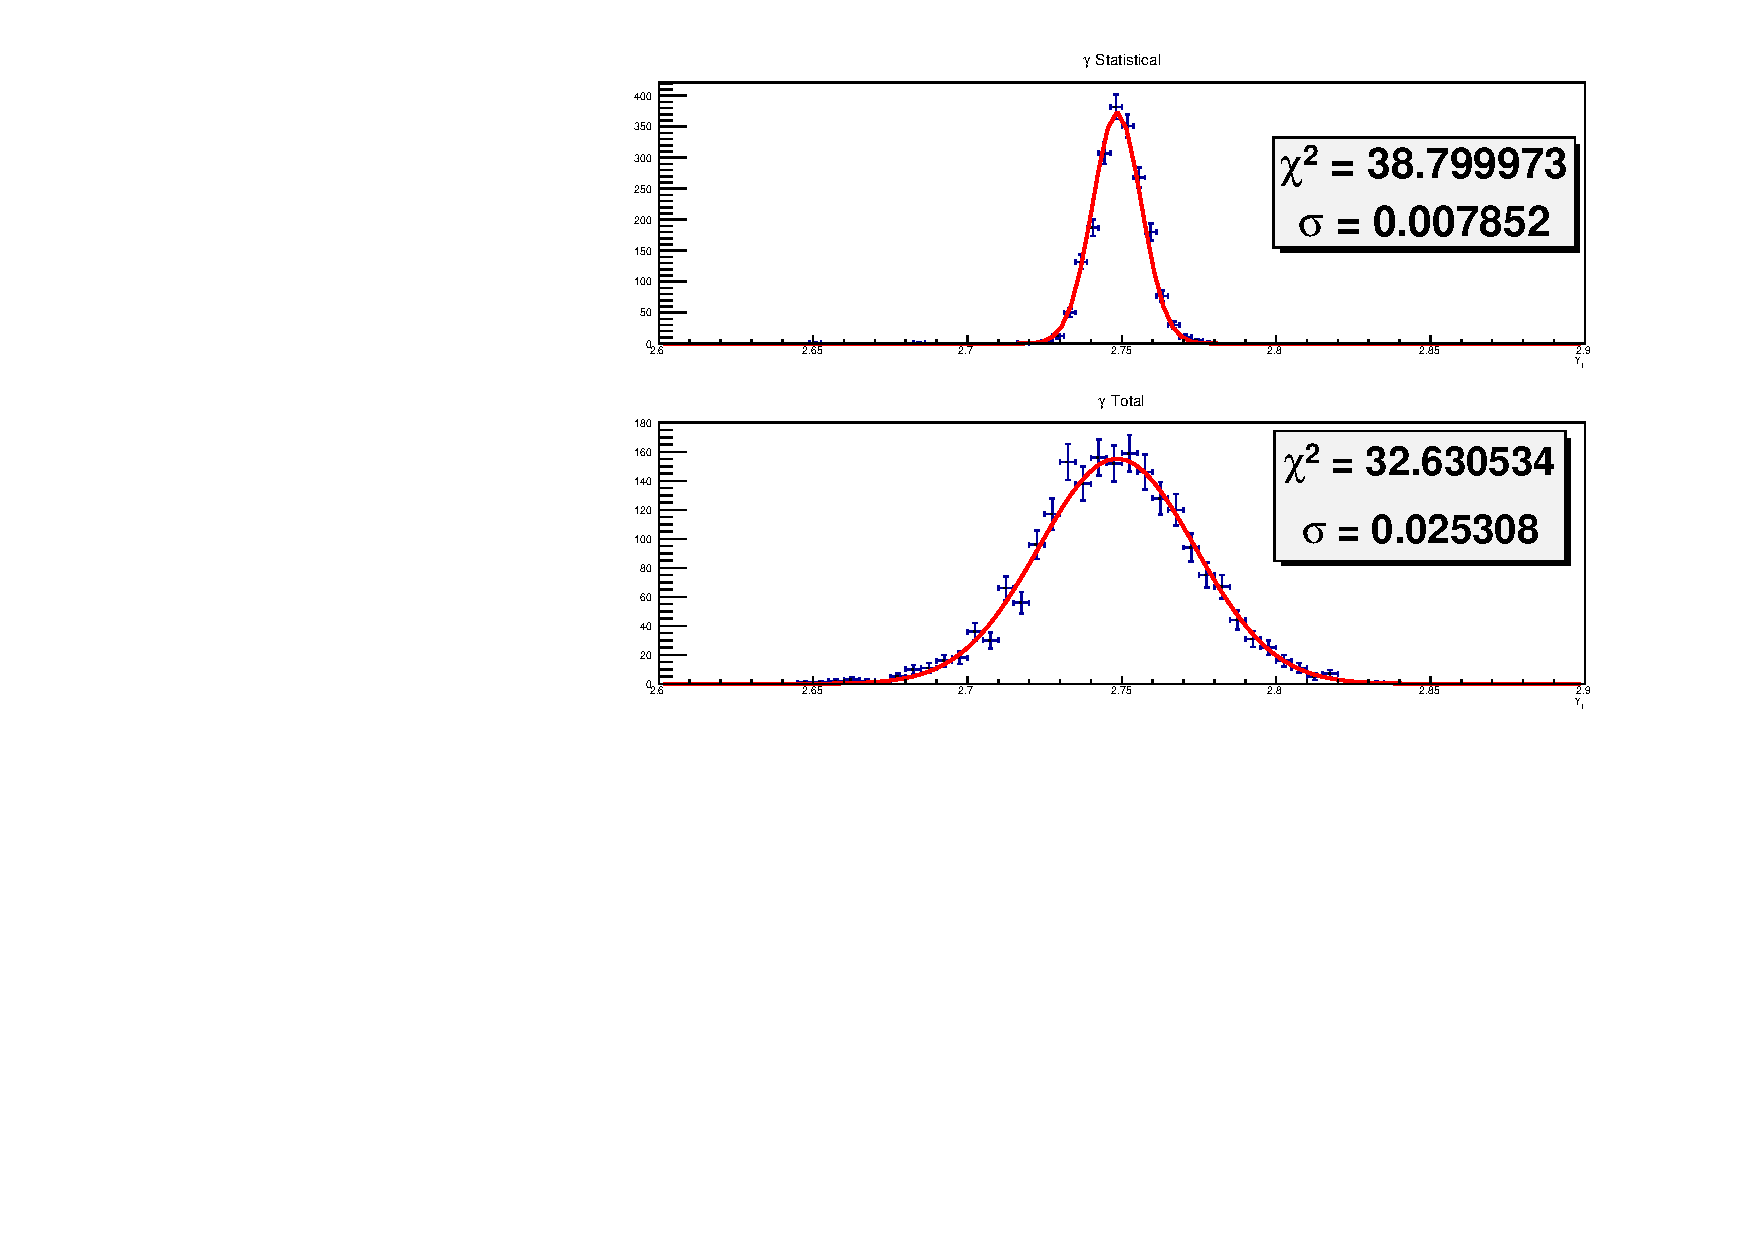
\includegraphics[width=0.8\textwidth]{SPL_Sim}};
% \node [opacity=0.2] (0,0) {\rotatebox{45}{\scalebox{3.0}{\textcolor{red}{preliminary}}}};
% \end{tikzpicture}
% \end{figure}

% \end{frame}
% %------ BPL ------
% \begin{frame}
% \frametitle{Broken power law (BPL)}

% %\begin{figure}[h!]
% %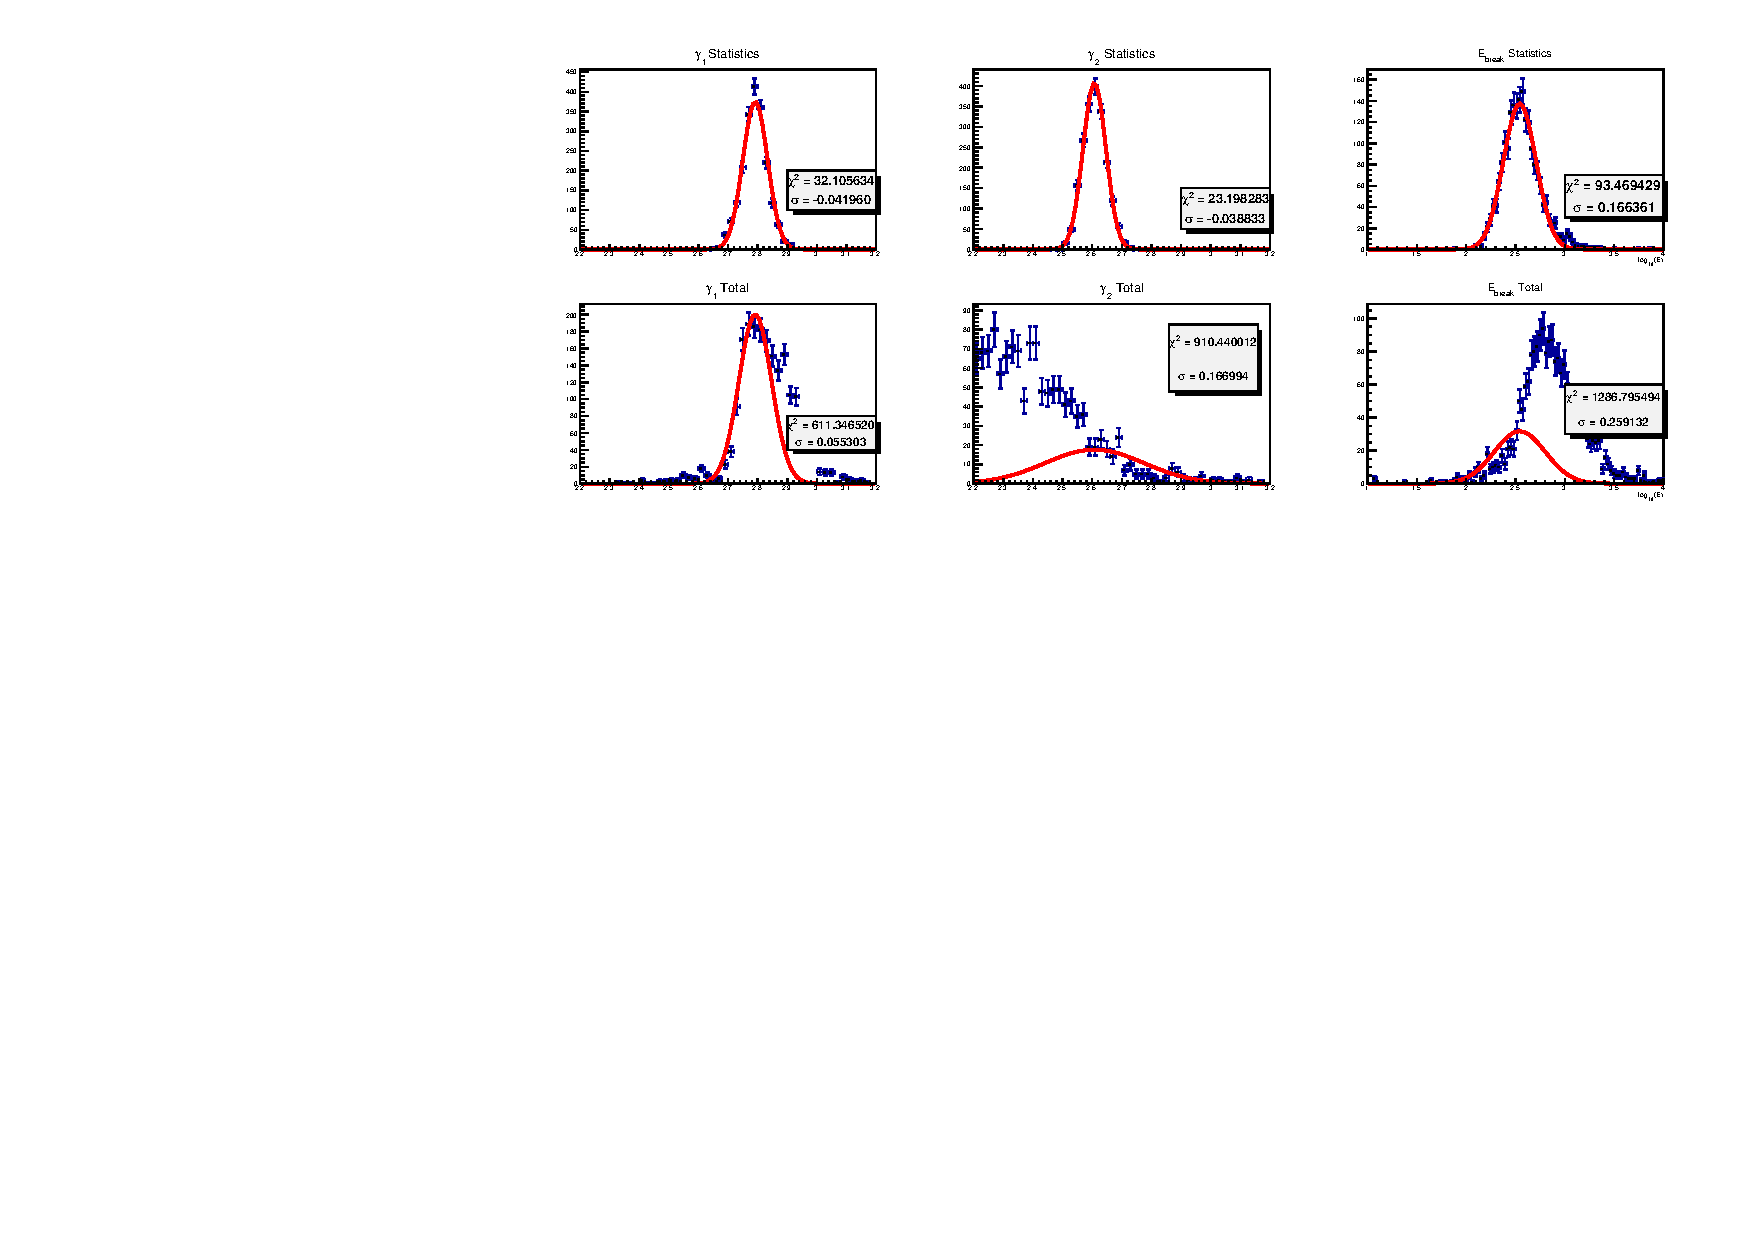
\includegraphics[width = \textwidth]{BPL_Sim}
% %\end{figure}

% \begin{figure}[h!]
% \begin{tikzpicture}
% \node (0,0) {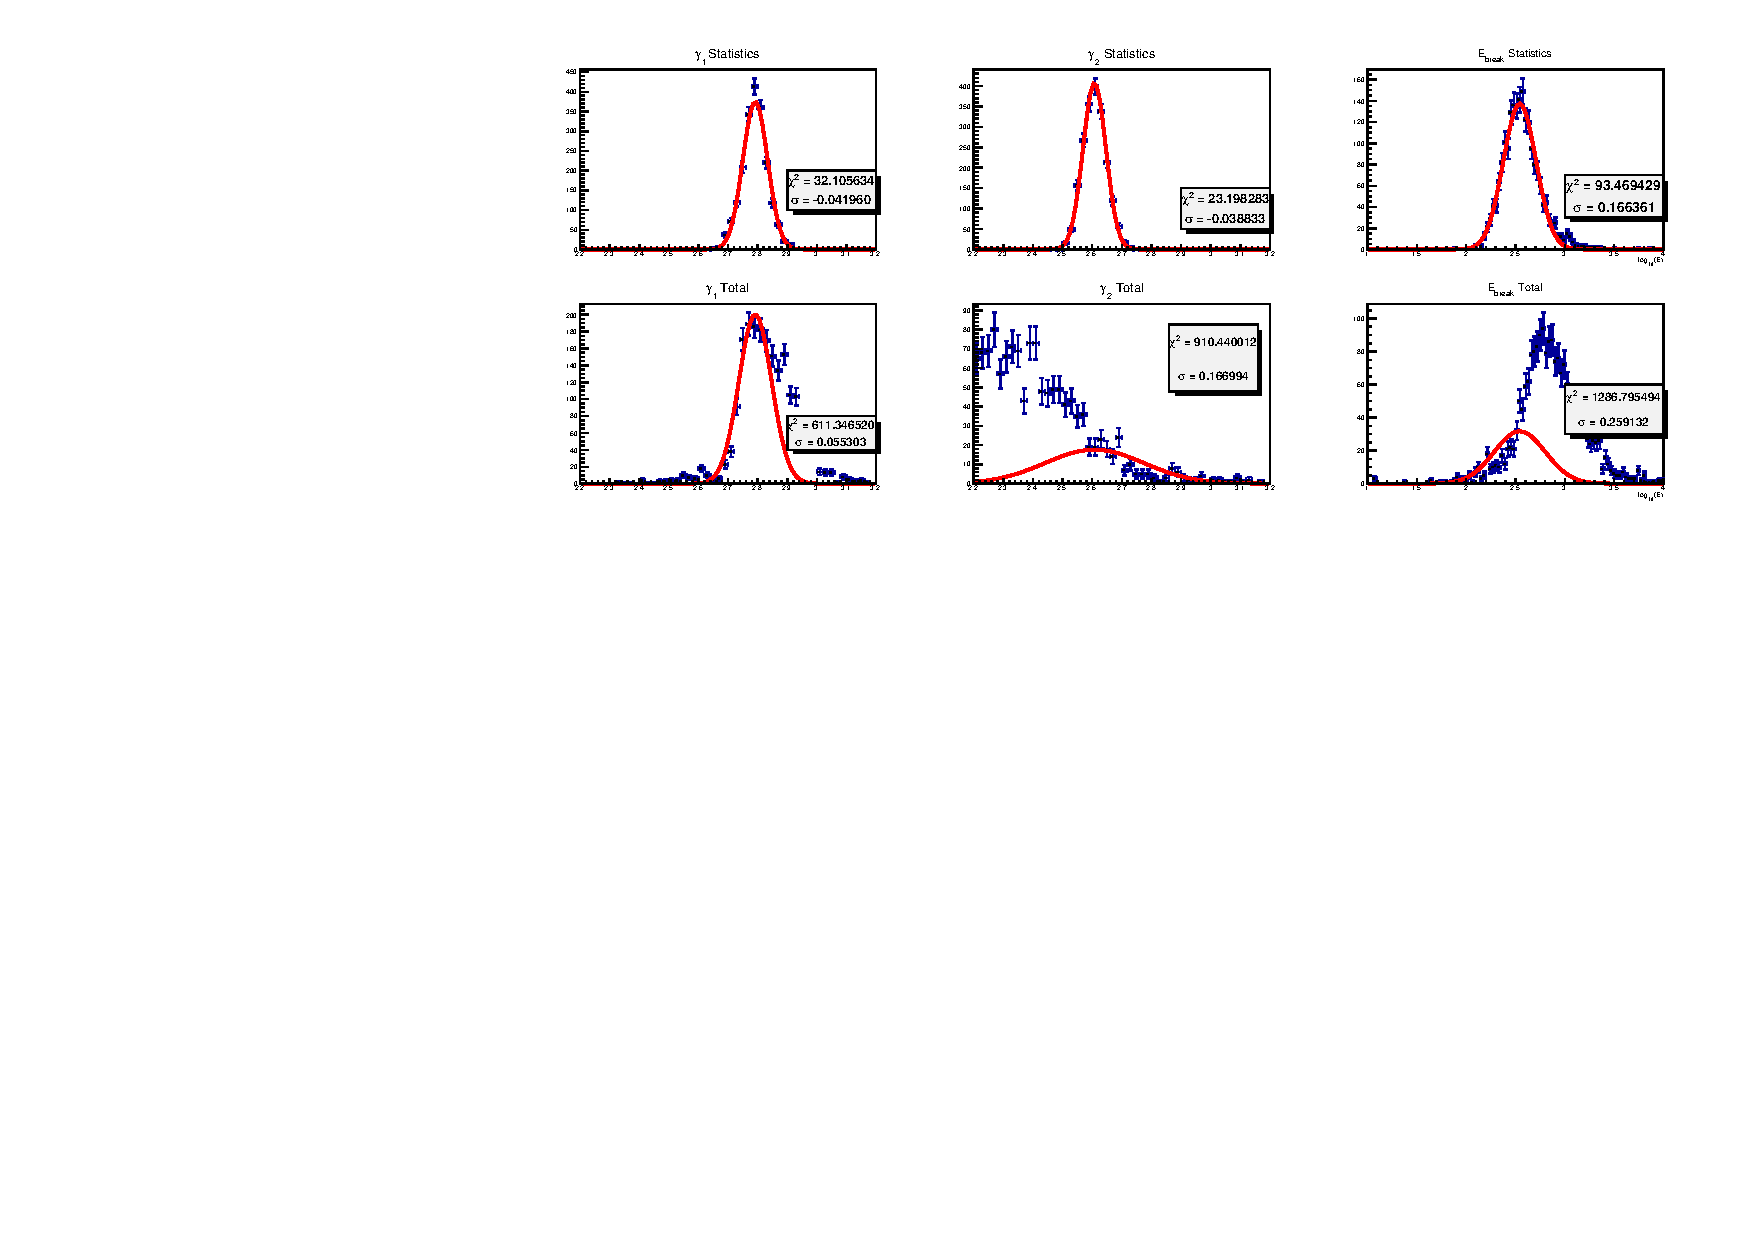
\includegraphics[width=\textwidth]{BPL_Sim}};
% \node [opacity=0.2] (0,0) {\rotatebox{25}{\scalebox{3.5}{\textcolor{red}{preliminary}}}};
% \end{tikzpicture}
% \end{figure}

% \end{frame}
% %------------------------------------------------
% %   4 )  To do list
% %------------------------------------------------
% \section{To do list}
% \begin{frame}
% \frametitle{To do}
% \begin{itemize}
% \item Problem of shifted value in BPL came from optimization algorithm because it stop in local minimum
% \item Extract new Flux due to technical problem (Still doubt.. might came from exposure map or photon selection)
% \item Fix bug in my log-likelihood function (Use count instread of flux)
% \item Resimulate data when I am done above stuff
% \end{itemize}
% \end{frame}

%------------------------------------------------
%   Conclusion
%------------------------------------------------
\section{Summary}
\begin{frame}
\frametitle{Conclusion}
\begin{itemize}
\item We found an energy break point around 328 GeV with a significant level of 3.3$\sigma$ which agree with other measurement
\item Put weight on the previous study [M. Ackermann et al. (2014)] that we could take a benefit of brightness $\gamma$-ray from Earth’s high atmosphere to indirectly observe cosmic ray spectrum which cause it's luminosity
\end{itemize}
\end{frame}


%------------------------------------------------


%------------------------------------------------
\section{} % just empty section for not showing header on slide

%------------------------------------------------
%    Reference
%------------------------------------------------
\section{Reference}
\begin{frame}
\frametitle{References}
[1] O. Adriani et al., Science 332, 69 (2011)
[2] M. Ackermann et al. (Fermi LAT Collaboration), Phys. Rev. Lett. 112, 151103 \newline
[3] Kachelriess $\&$ Ostapchenko, Phys. Rev. D 86 \newline
[4] M. Aguilar et al. (AMS Collaboration), Phys. Rev. Lett. 115, 211101 \newline
[5] M. Aguilar et al. (AMS Collaboration), Phys. Rev. Lett. 114, 171103 \newline
[6] L. Lyons, Statistics for nuclear and particle physicists
\end{frame}
%------------------------------------------------
%    Acknowledgement
%------------------------------------------------
\section{}
\begin{frame}\frametitle{Acknowledgement}
  \begin{itemize}
    \item Dr. Warit Mitthumsiri \\ Mahidol University, Thailand
    \item Dr. Francesca Spada \\ University of Pisa, Italy
    \item People in the Space Physics laboratory at Mahidol University and the Fermi lab at the University of Pisa
    \item Development and Promotion of Science and Technology Talents Project (DPST)
    \item Partially supported by the Thailand Research Fund Award RTA5980003
  \end{itemize}
\end{frame}

%------------------------------------------------
%    Back up slide
%------------------------------------------------

\begin{frame}
\Huge{\centerline{Backup slide}}
\end{frame}

% % ------- poewr law in rigidity -------------
% \begin{frame}
% \frametitle{Power law (in rigidity)}
% Typically, cosmic ray spectrum follow power law in rigidity as \\
% \textbf{Single power law (SPL)}
% \begin{equation}
% \frac{dN}{dR} = R_0R^{-\gamma}
% \end{equation}
% \textbf{Broken power law (BPL)}
% \begin{equation}
% \frac{dN}{dR}=
%   \begin{cases}
%     R_0R^{-\gamma_1}\ :\ E < E_{\text{Break}}\\
%     R_0[R(E_{\text{Break}})]^{\gamma_2-\gamma_1}R^{-\gamma_2}\ :\ E \ge E_{\text{Break}}
%   \end{cases}
% \end{equation}
% Note for someone who not famoliar with rigidity : it just defined by $R\equiv P/q$ when $P, q$ is a momentum and charge of particle
% \end{frame}
% ------- power law in Energy -------------
\begin{frame}
\frametitle{Power law in energy}
In our case, we use power in energy then we need to convert by relativistic energy-mass relation \\
\textbf{Single power law (SPL)}
\begin{equation}
\frac{dN}{dE} = N_0[E_k(E_k+2m_p)]^{-\gamma/2} \left(\frac{E_k+m_p}{\sqrt{E_k(E_k+2m_p)}}\right)
\end{equation}
\textbf{Broken power law (BPL)}
\begin{equation}
\frac{dN}{dE}=
  \begin{cases}
    N_0[E_k(E_k+2m_p)]^{-\gamma_1/2} \left(\frac{E_k+m_p}{\sqrt{E_k(E_k+2m_p)}}\right)\ :\ E < E_{\text{Break}}\\
    N_0[E_b(E_b+2m_p)]^{(\gamma_2-\gamma_1)/2}[E_k(E_k+2m_p)]^{-\gamma_2/2} \left(\frac{E_k+m_p}{\sqrt{E_k(E_k+2m_p)}}\right)\\ :\ E \ge E_{\text{Break}}
  \end{cases}
\end{equation}
\end{frame}
%----------------------------------
% -----  Error determination --------
%----------------------------------
%----- How to deal with this ?
\begin{frame}
  \frametitle{Error determination}
  \textbf{Statictical error (Random error)}
  \begin{enumerate}
    \item Get back to raw count and
    \textcolor{blue}{random new count in each energy bin by Poisson random function}
    \item Recalculate proton spectrum
    \item Optimize it and store the parameter that we got
    \item do it over thoundsand time and fill in histogram to interpret error by saying sigma of gaussian function
  \end{enumerate}
  \textbf{Total error (take into account instrument)}
  \begin{enumerate}
    \item Get back to raw count and
    \textcolor{blue}{random new count in each energy bin by Poisson random function}
    \item \textcolor{blue}{Random value we got again by systematic error (Apparatus)}
    \item Recalculate proton spectrum
    \item Optimize it and store the parameter that we got
    \item do it over thoundsand time and fill in histogram to interpret error by saying sigma of gaussian function
  \end{enumerate}
  \end{frame}
  
  \begin{frame}\frametitle{Monte Carlo Simulation}
    \begin{figure}[h!]
      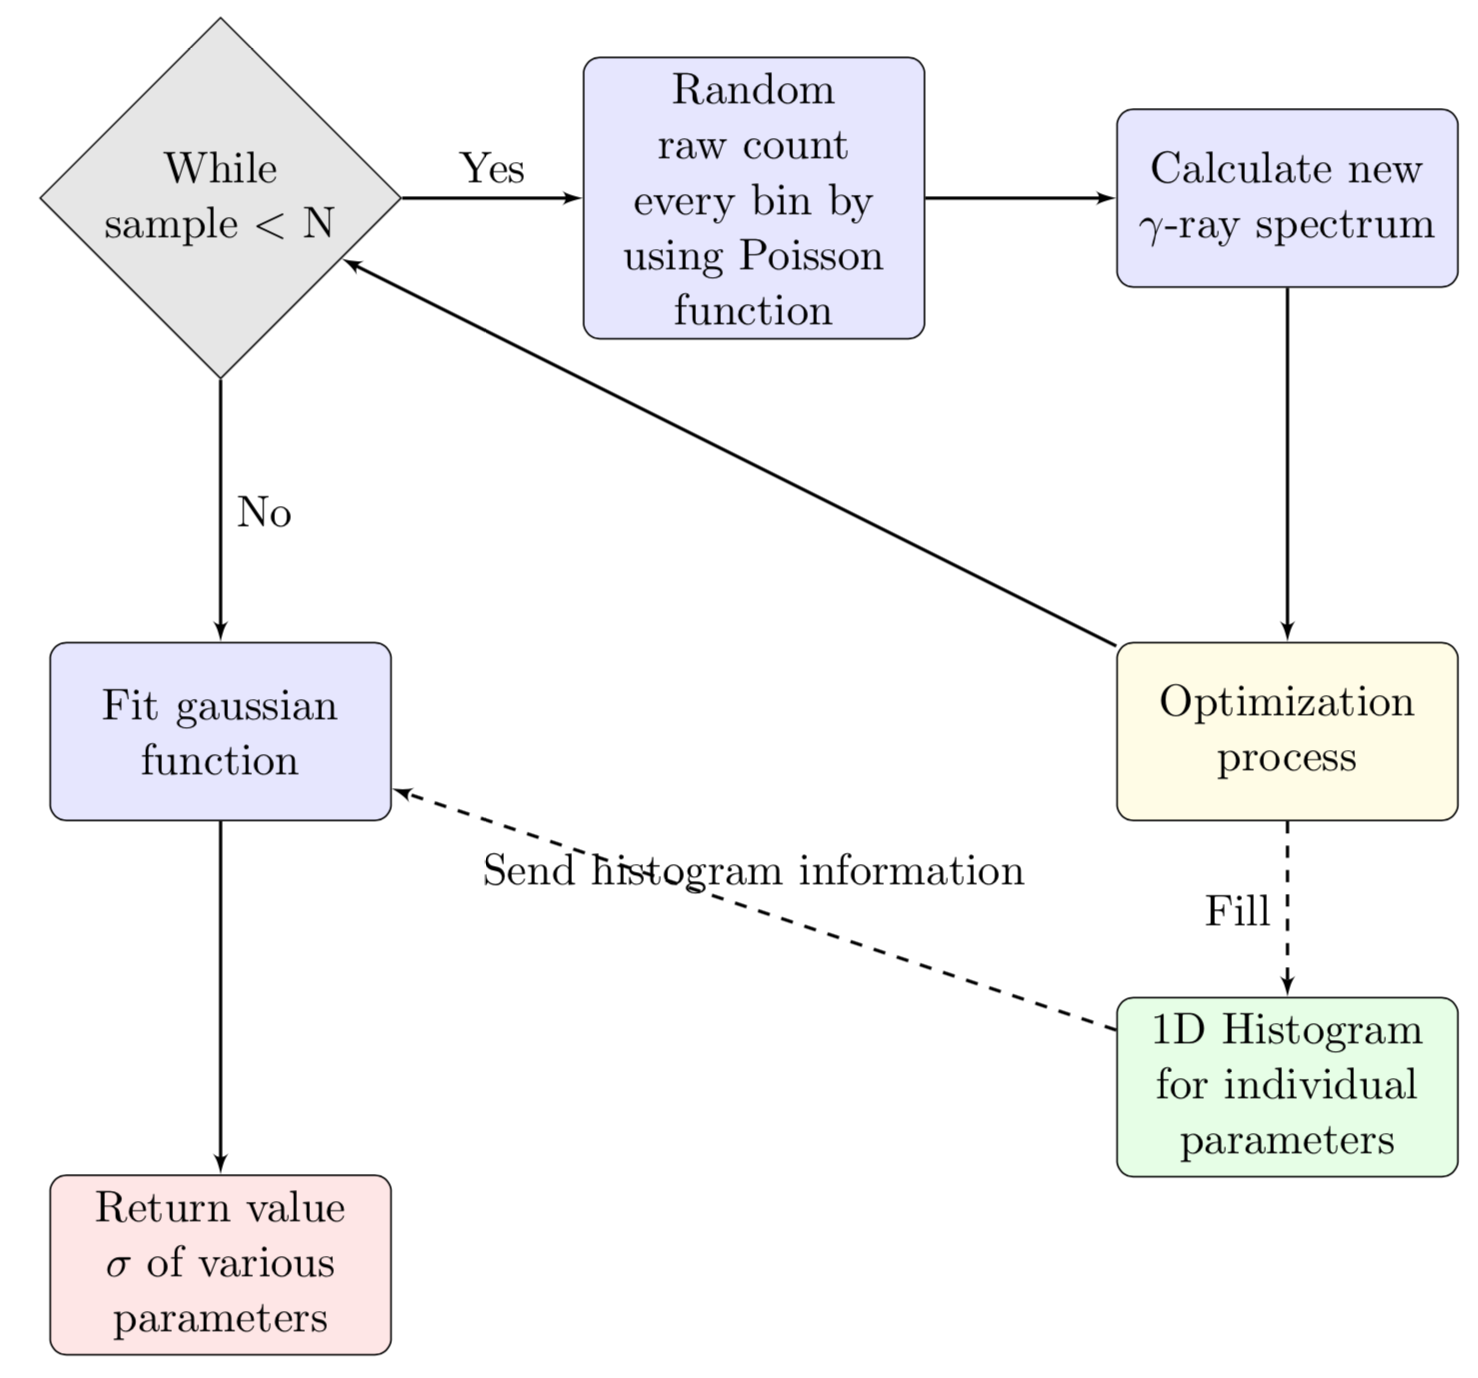
\includegraphics[width=0.7\textheight]{montestat}
      \caption{Statictical error determination}
      \end{figure}
  \end{frame}

  \begin{frame}\frametitle{Monte Carlo Simulation}
    \begin{figure}[h!]
      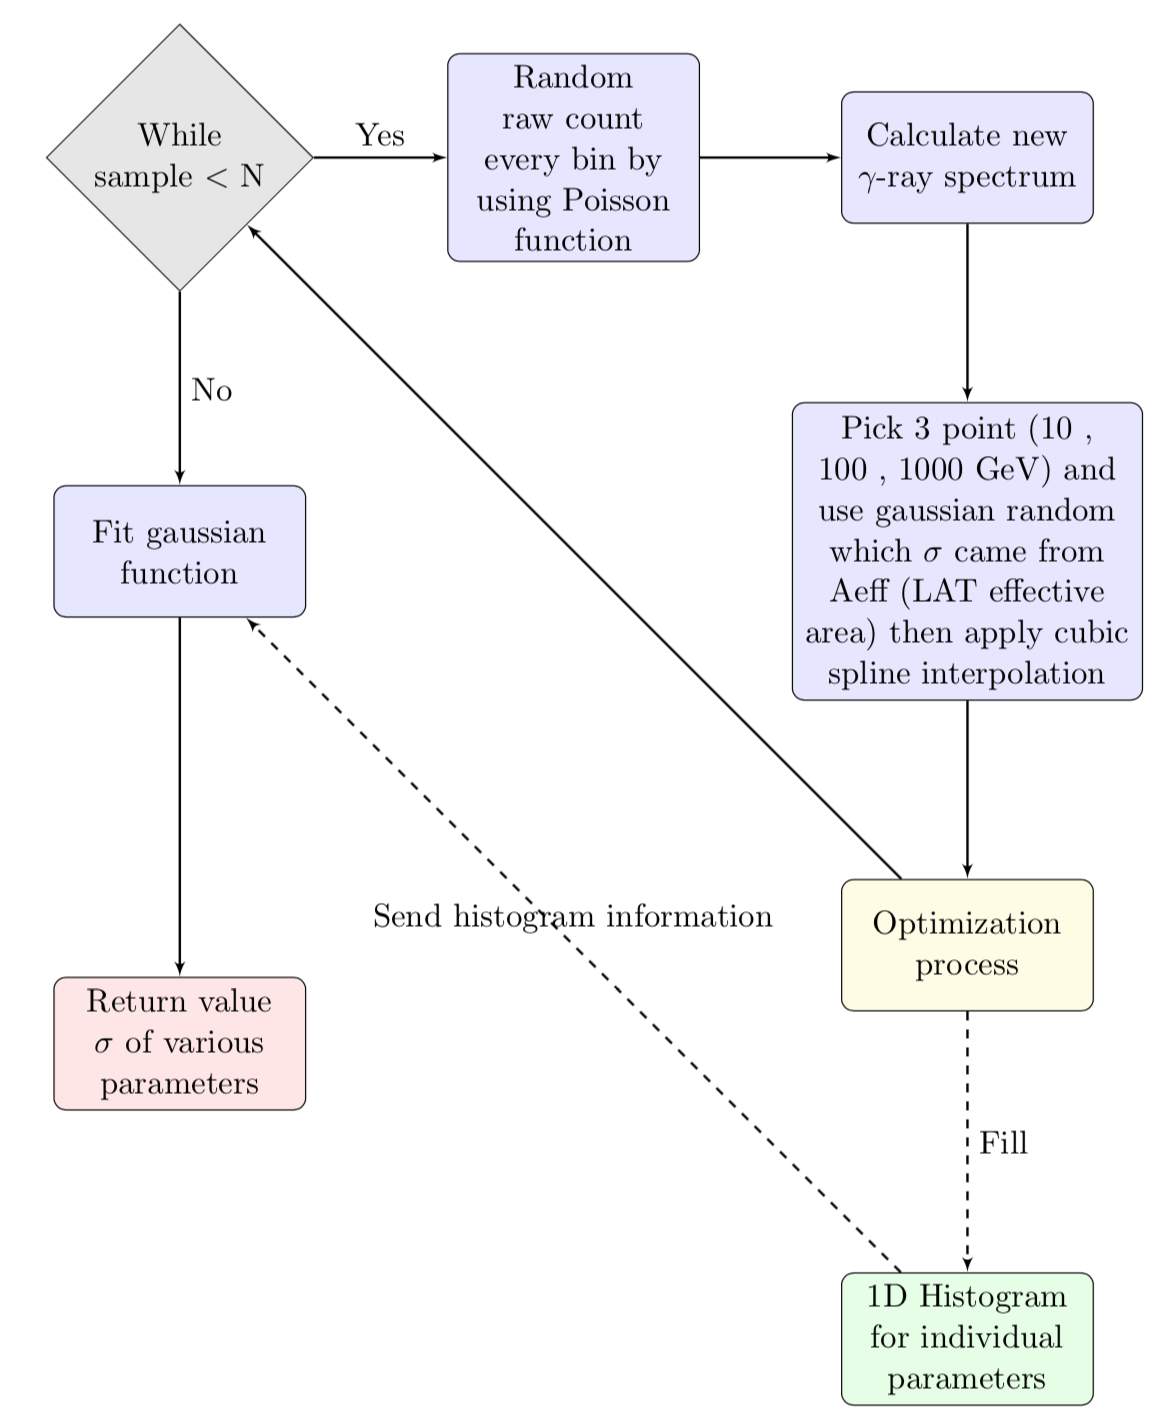
\includegraphics[width=0.65\textheight]{montetot}
      \caption{Total error determination}
      \end{figure}
  \end{frame}

  %----- SPL ------
  \begin{frame}
  \frametitle{Single power law (SPL)}
  
  \begin{figure}[h!]
  \begin{tikzpicture}
  \node (0,0) {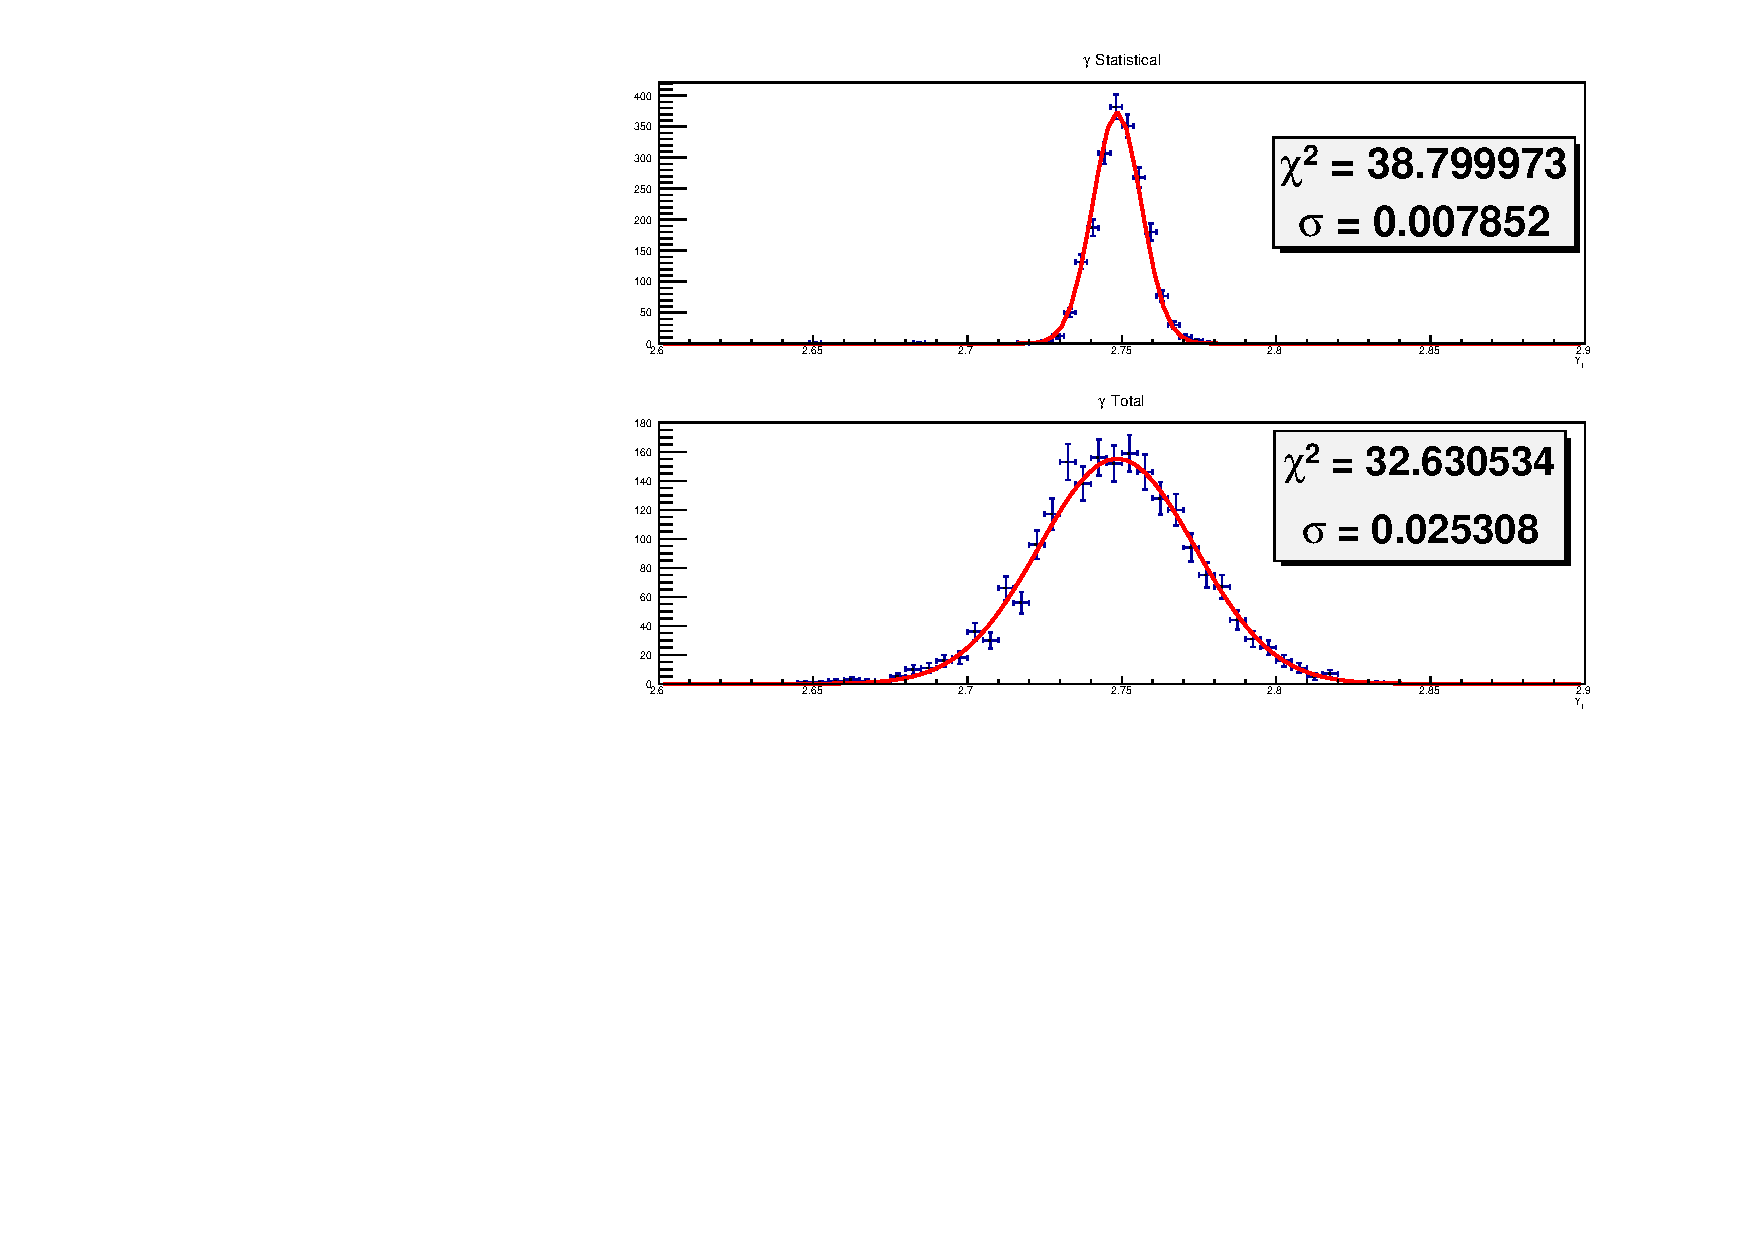
\includegraphics[width=0.8\textwidth]{SPL_Sim}};
  \node [opacity=0.2] (0,0) {\rotatebox{45}{\scalebox{3.0}{\textcolor{red}{preliminary}}}};
  \end{tikzpicture}
  \end{figure}
  
  \end{frame}
  %------ BPL ------
  \begin{frame}
  \frametitle{Broken power law (BPL)}
  
  %\begin{figure}[h!]
  %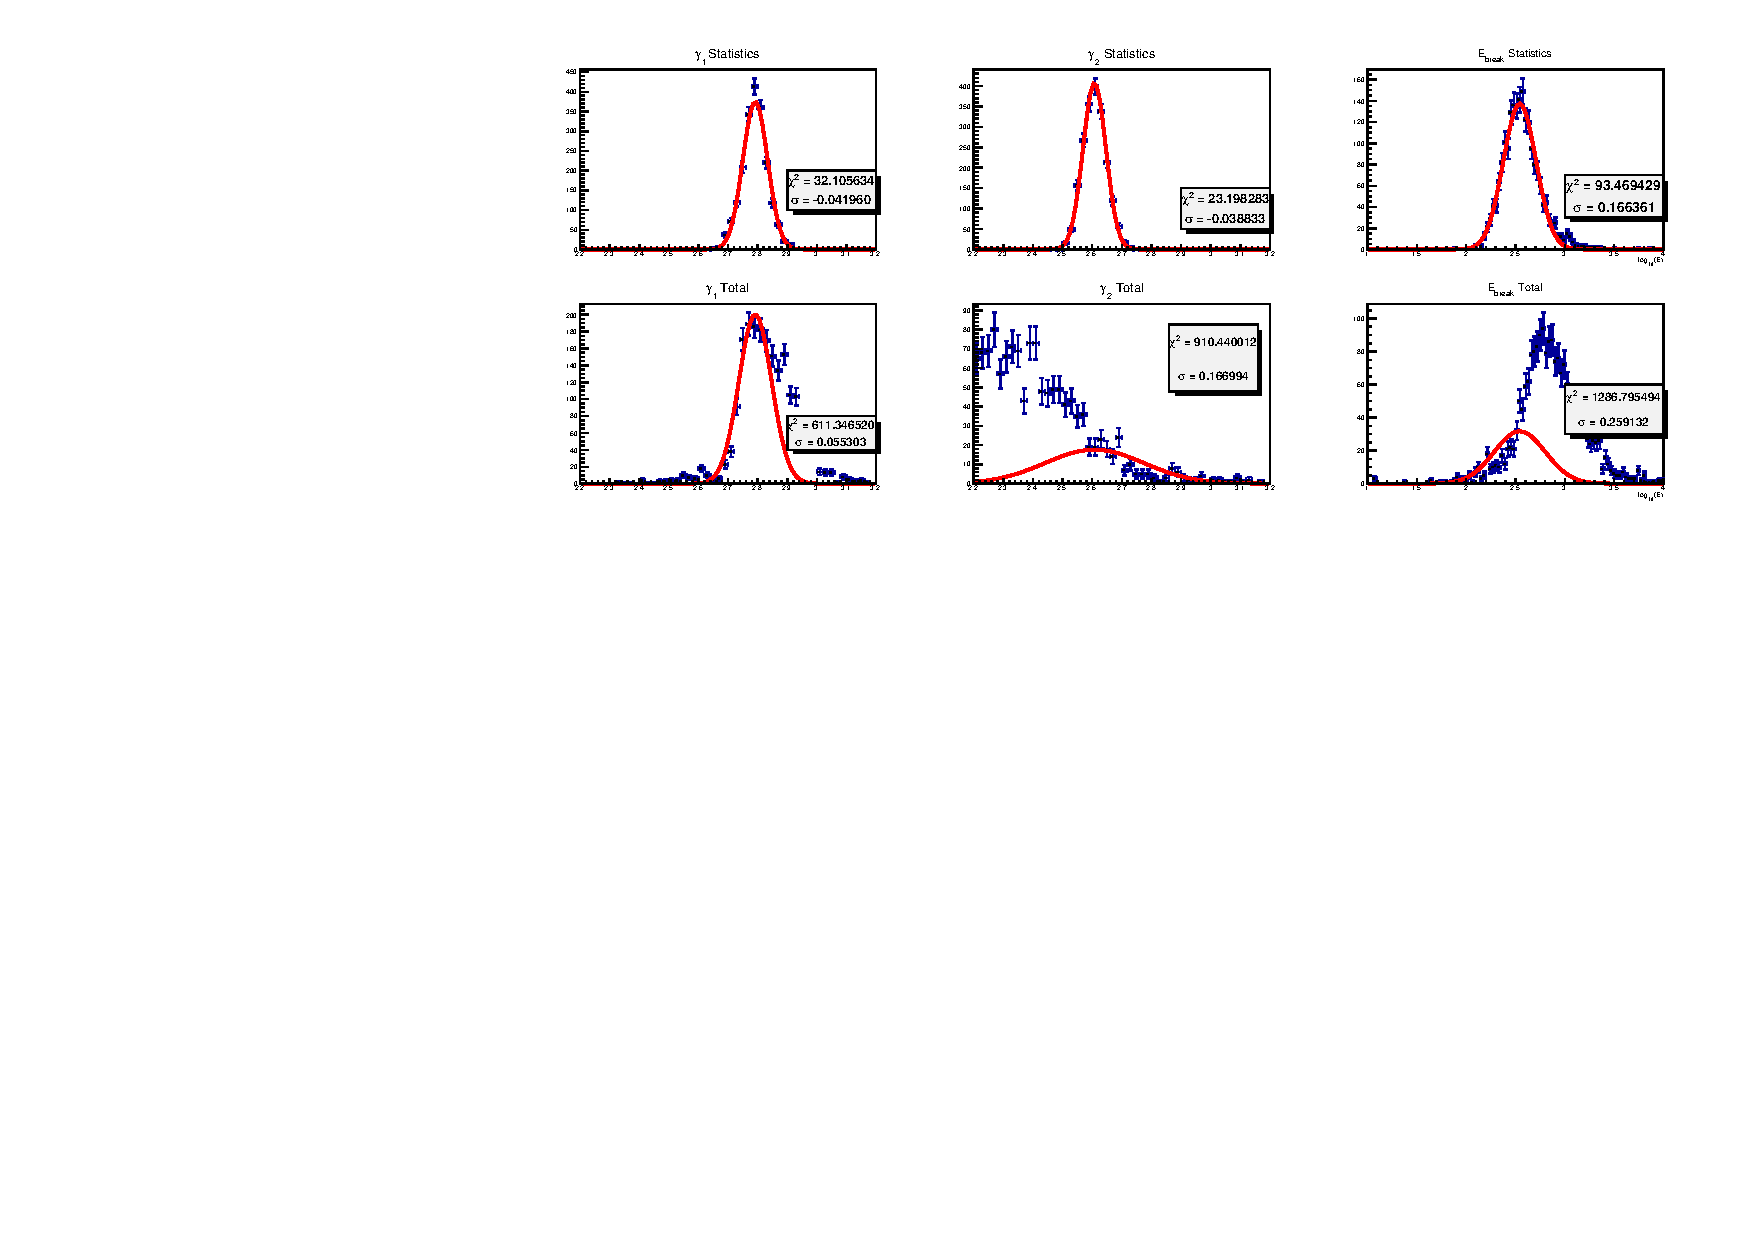
\includegraphics[width = \textwidth]{BPL_Sim}
  %\end{figure}
  
  \begin{figure}[h!]
  \begin{tikzpicture}
  \node (0,0) {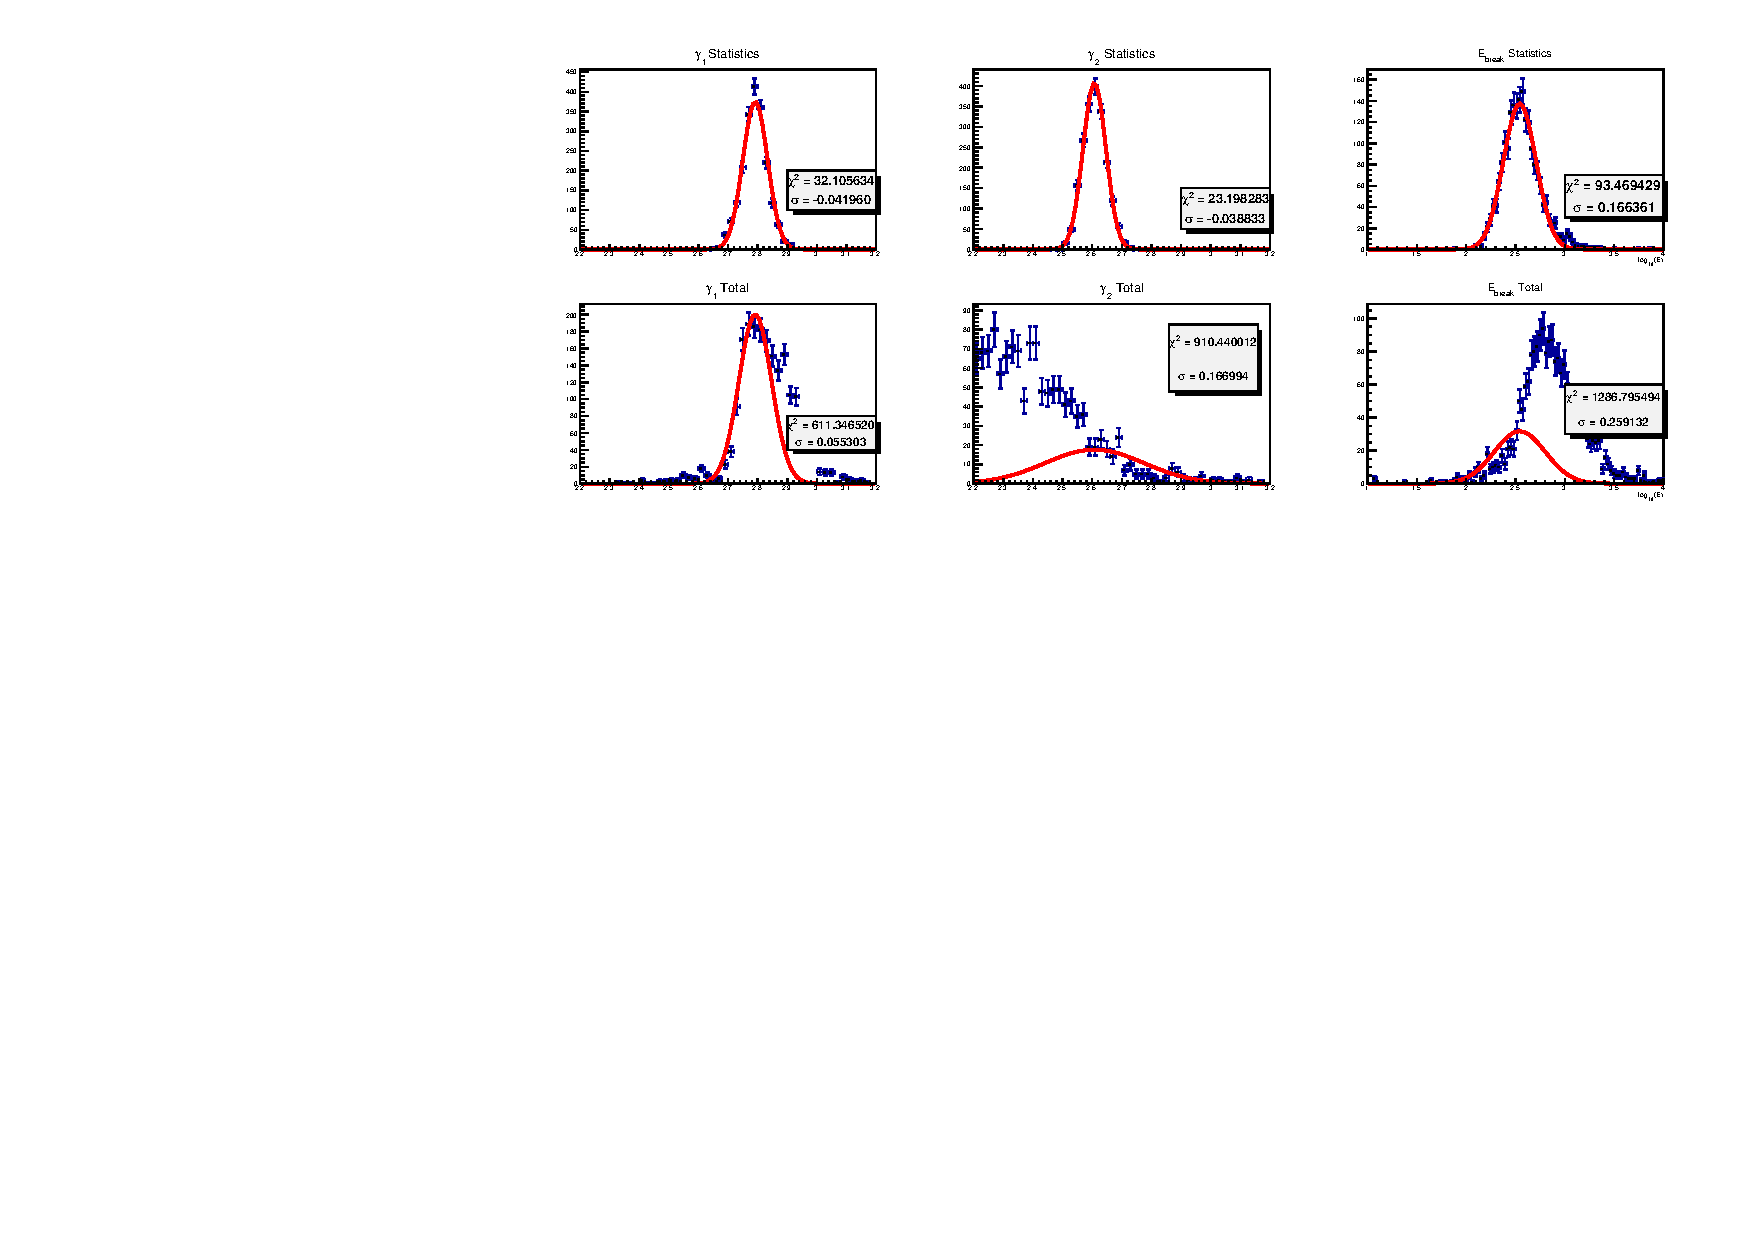
\includegraphics[width=\textwidth]{BPL_Sim}};
  \node [opacity=0.2] (0,0) {\rotatebox{25}{\scalebox{3.5}{\textcolor{red}{preliminary}}}};
  \end{tikzpicture}
  \end{figure}
  
  \end{frame}

%----------------------------------
% ---------  calculation map --------
%----------------------------------
%--- cntmap ---
\begin{frame}
\frametitle{Count map}

%\begin{figure}[h!]
%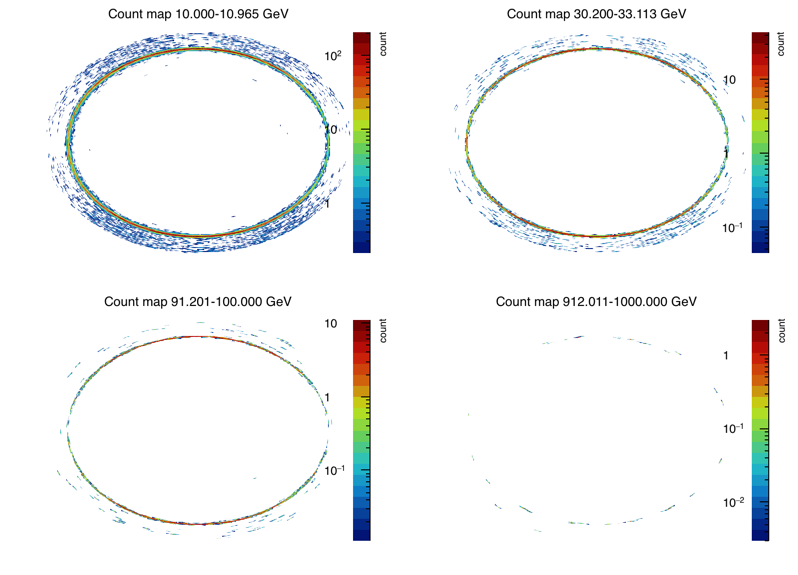
\includegraphics[width = 0.9\textwidth]{cntmap}
%\caption{Bla1}
%\end{figure}

\begin{figure}[h!]
\begin{tikzpicture}
\node (0,0) {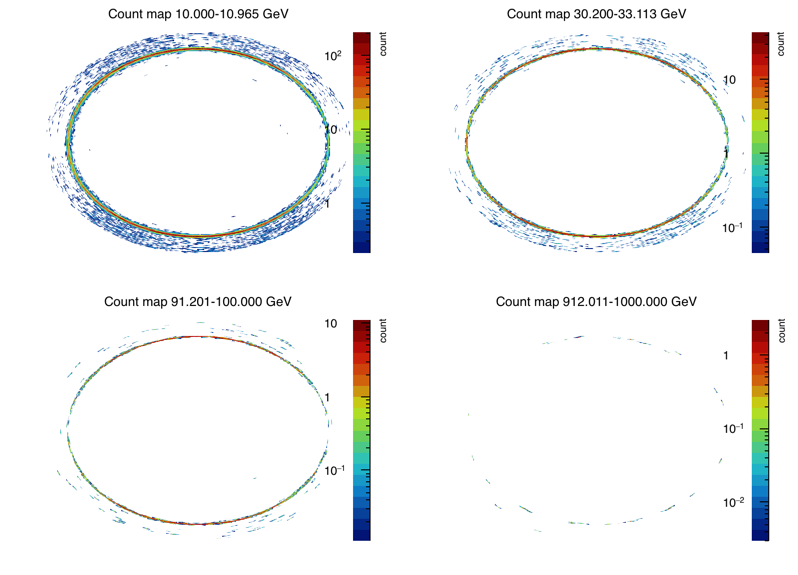
\includegraphics[width=0.9\textwidth]{cntmap}};
\node [opacity=0.2] (0,0) {\rotatebox{45}{\scalebox{3.5}{\textcolor{red}{preliminary}}}};
\end{tikzpicture}
\end{figure}

\end{frame}
%--- expmap ---
\begin{frame}
\frametitle{Exposure map}

%\begin{figure}[h!]
%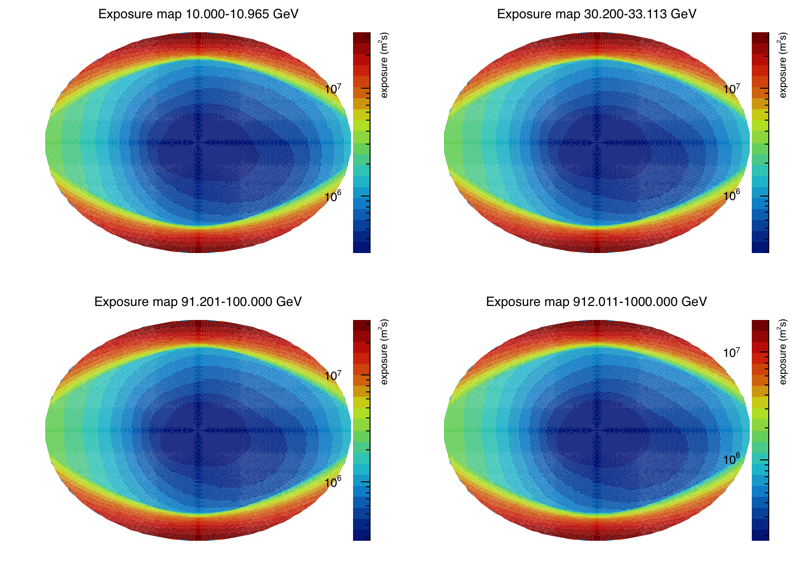
\includegraphics[width = 0.9\textwidth]{expmap}
%\caption{Bla1}
%\end{figure}

\begin{figure}[h!]
\begin{tikzpicture}
\node (0,0) {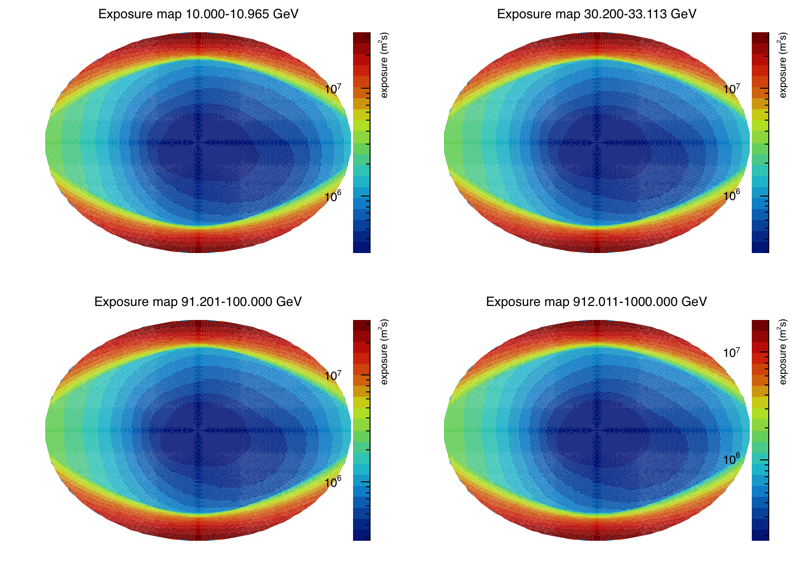
\includegraphics[width=0.9\textwidth]{expmap}};
\node [opacity=0.2] (0,0) {\rotatebox{45}{\scalebox{3.5}{\textcolor{red}{preliminary}}}};
\end{tikzpicture}
\end{figure}

\end{frame}
%--- flxmap ---
\begin{frame}
\frametitle{Flux map}

%\begin{figure}[h!]
%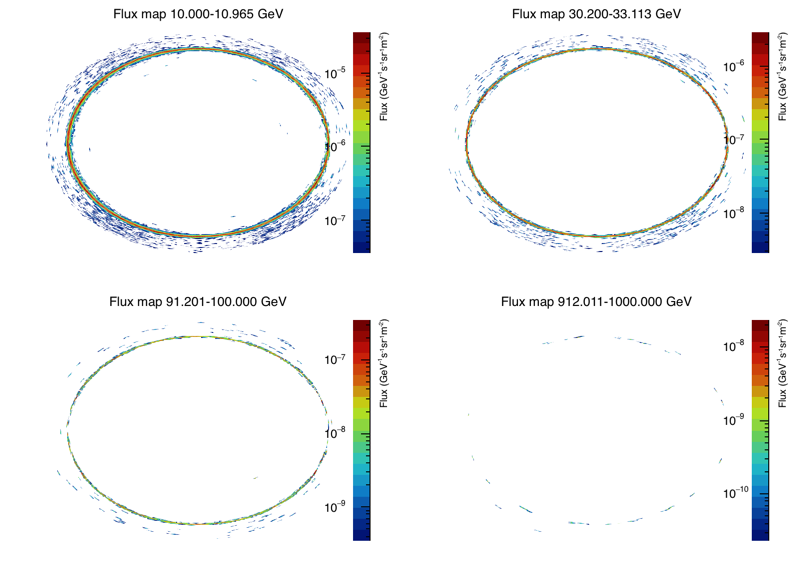
\includegraphics[width = 0.9\textwidth]{flxmap}
%\caption{Bla1}
%\end{figure}

\begin{figure}[h!]
\begin{tikzpicture}
\node (0,0) {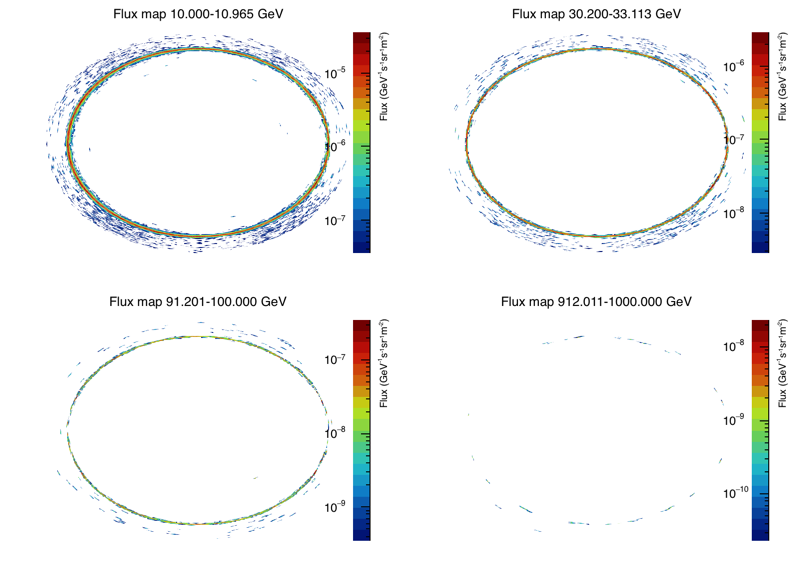
\includegraphics[width=0.9\textwidth]{flxmap}};
\node [opacity=0.2] (0,0) {\rotatebox{45}{\scalebox{3.5}{\textcolor{red}{preliminary}}}};
\end{tikzpicture}
\end{figure}
\end{frame}

% \end{frame}

%----------------------------------------------------------------------------------------

\end{document}
